\documentclass[11pt]{article}
\usepackage[utf8]{inputenc}	% Para caracteres en español
\usepackage{amsmath,amsthm,amsfonts,amssymb,amscd}
\usepackage{multirow,booktabs}
\usepackage[dvipsnames]{xcolor}
\usepackage{fullpage}
\usepackage{lastpage}
\usepackage{enumitem}
\usepackage{fancyhdr}
\usepackage{mathrsfs}
\usepackage{wrapfig}
\usepackage{setspace}
\usepackage{calc}
\usepackage{multicol}
\usepackage{cancel}
\usepackage{currency}
\DefineCurrency{GBP}{name={pound},plural={pounds},iso={GBP},kind=iso,symbol={\£}}
\usepackage[retainorgcmds]{IEEEtrantools}
\usepackage[margin=3cm]{geometry}
\usepackage{amsmath}
\newlength{\tabcont}
\setlength{\parindent}{0.0in}
\setlength{\parskip}{0.05in}
\usepackage{empheq}
\usepackage{framed}
\usepackage[most]{tcolorbox}
\usepackage{xcolor}
%\usepackage[demo]{graphicx}
\usepackage{subfig}
\usepackage{mdframed}
\usepackage{biblatex}
\addbibresource{bib.bib}
\usepackage{hyperref}
\usepackage{soul}


\colorlet{shadecolor}{orange!15}
\parindent 0in
\parskip 12pt
\geometry{margin=1in, headsep=0.25in}
\theoremstyle{definition}
\newtheorem{reg}{Rule}

\newtheoremstyle{mystyle}{}{}{}{}{\sffamily\bfseries}{.}{ }{}
\newtheoremstyle{cstyle}{}{}{}{}{\sffamily\bfseries}{.}{ }{\thmnote{#3}}
\makeatletter
\renewenvironment{proof}[1][\proofname] {\par\pushQED{\qed}{\normalfont\sffamily\bfseries\topsep6\p@\@plus6\p@\relax #1\@addpunct{.} }}{\popQED\endtrivlist\@endpefalse}
\makeatother

\theoremstyle{mystyle}{\newtheorem{definition}{Definition}[section]}
\theoremstyle{mystyle}{\newtheorem*{note}{Note}}
\theoremstyle{mystyle}{\newtheorem*{example}{Example}}
\theoremstyle{mystyle}{\newtheorem*{deriv}{Derivation}}
\theoremstyle{mystyle}{\newtheorem*{intu}{Intuition}}

\tcolorboxenvironment{example}{boxrule=0pt,boxsep=0pt,blanker,borderline west={2pt}{0pt}{black},left=8pt,right=8pt,sharp corners,before skip=10pt,after skip=10pt,breakable}
\tcolorboxenvironment{definition}{boxrule=0pt,boxsep=0pt,colback={red!10},left=8pt,right=8pt,enhanced jigsaw, borderline west={2pt}{0pt}{red},sharp corners,before skip=10pt,after skip=10pt,breakable}
\tcolorboxenvironment{note}{boxrule=0pt,boxsep=0pt,blanker,borderline west={2pt}{0pt}{green},left=8pt,right=8pt,before skip=10pt,after skip=10pt,breakable}
\tcolorboxenvironment{deriv}{boxrule=0pt,boxsep=0pt,colback={blue!10},left=8pt,right=8pt,enhanced jigsaw, borderline west={2pt}{0pt}{blue},sharp corners,before skip=10pt,after skip=10pt,breakable}
\tcolorboxenvironment{intu}{boxrule=0pt,boxsep=0pt,blanker,borderline west={2pt}{0pt}{pink},left=8pt,right=8pt,before skip=10pt,after skip=10pt,breakable}


\definecolor{codeblue}{rgb}{0.29296875, 0.51953125, 0.68359375}
\definecolor{codegreen}{rgb}{0.47265625, 0.62890625, 0.40234375}
\definecolor{codegray}{rgb}{0.95703125, 0.95703125, 0.95703125}
\definecolor{codecrimson}{rgb}{0.87109375,0.3984375,0.3984375}
\definecolor{contcol1}{HTML}{FFC7C7}
\definecolor{contcol2}{HTML}{9EF5A3}
\setcounter{tocdepth}{2}

\lstset{frame=tb,
  backgroundcolor=\color{codegray},
  aboveskip=3mm,
  belowskip=3mm,
  showstringspaces=false,
  columns=flexible,
  basicstyle={\ttfamily},
  numbers=left,
  numberstyle=\tiny\color{gray},
  keywordstyle=\color{codeblue},
  commentstyle=\color{codegreen},
  stringstyle=\color{codecrimson},
  breaklines=true,
  breakatwhitespace=true,
  tabsize=4,
  frame=tlbr,framesep=4pt,framerule=0pt,
  escapeinside = ''
}

\usepackage{listings}

% language definition
\lstdefinelanguage{Stata}{
    % System commands
    morekeywords=[1]{regress, reg, summarize, sum, display, di, generate, gen, bysort, use, import, delimited, predict, quietly, probit, margins, test, ivregress, 2sls, xtset, xtreg, nl},
    % Reserved words
    morekeywords=[2]{aggregate, array, boolean, break, byte, case, catch, class, colvector, complex, const, continue, default, delegate, delete, do, double, else, eltypedef, end, enum, explicit, export, external, float, for, friend, function, global, goto, if, inline, int, local, long, mata, matrix, namespace, new, numeric, NULL, operator, orgtypedef, pointer, polymorphic, pragma, private, protected, public, quad, real, return, rowvector, scalar, short, signed, static, strL, string, struct, super, switch, template, this, throw, transmorphic, try, typedef, typename, union, unsigned, using, vector, version, virtual, void, volatile, while,},
    % Keywords
    morekeywords=[3]{forvalues, foreach, set},
    % Date and time functions
    morekeywords=[4]{bofd, Cdhms, Chms, Clock, clock, Cmdyhms, Cofc, cofC, Cofd, cofd, daily, date, day, dhms, dofb, dofC, dofc, dofh, dofm, dofq, dofw, dofy, dow, doy, halfyear, halfyearly, hh, hhC, hms, hofd, hours, mdy, mdyhms, minutes, mm, mmC, mofd, month, monthly, msofhours, msofminutes, msofseconds, qofd, quarter, quarterly, seconds, ss, ssC, tC, tc, td, th, tm, tq, tw, week, weekly, wofd, year, yearly, yh, ym, yofd, yq, yw,},
    % Mathematical functions
    morekeywords=[5]{abs, ceil, cloglog, comb, digamma, exp, expm1, floor, int, invcloglog, invlogit, ln, ln1m, ln, ln1p, ln, lnfactorial, lngamma, log, log10, log1m, log1p, logit, max, min, mod, reldif, round, sign, sqrt, sum, trigamma, trunc,},
    % Matrix functions
    morekeywords=[6]{cholesky, coleqnumb, colnfreeparms, colnumb, colsof, corr, det, diag, diag0cnt, el, get, hadamard, I, inv, invsym, issymmetric, J, matmissing, matuniform, mreldif, nullmat, roweqnumb, rownfreeparms, rownumb, rowsof, sweep, trace, vec, vecdiag, },
    % Programming functions
    morekeywords=[7]{autocode, byteorder, c, _caller, chop, abs, clip, cond, e, fileexists, fileread, filereaderror, filewrite, float, fmtwidth, has_eprop, inlist, inrange, irecode, matrix, maxbyte, maxdouble, maxfloat, maxint, maxlong, mi, minbyte, mindouble, minfloat, minint, minlong, missing, r, recode, replay, return, s, scalar, smallestdouble,},
    % Random-number functions
    morekeywords=[8]{rbeta, rbinomial, rcauchy, rchi2, rexponential, rgamma, rhypergeometric, rigaussian, rlaplace, rlogistic, rnbinomial, rnormal, rpoisson, rt, runiform, runiformint, rweibull, rweibullph,},
    % Selecting time-span functions
    morekeywords=[9]{tin, twithin,},
    % Statistical functions
    morekeywords=[10]{betaden, binomial, binomialp, binomialtail, binormal, cauchy, cauchyden, cauchytail, chi2, chi2den, chi2tail, dgammapda, dgammapdada, dgammapdadx, dgammapdx, dgammapdxdx, dunnettprob, exponential, exponentialden, exponentialtail, F, Fden, Ftail, gammaden, gammap, gammaptail, hypergeometric, hypergeometricp, ibeta, ibetatail, igaussian, igaussianden, igaussiantail, invbinomial, invbinomialtail, invcauchy, invcauchytail, invchi2, invchi2tail, invdunnettprob, invexponential, invexponentialtail, invF, invFtail, invgammap, invgammaptail, invibeta, invibetatail, invigaussian, invigaussiantail, invlaplace, invlaplacetail, invlogistic, invlogistictail, invnbinomial, invnbinomialtail, invnchi2, invnF, invnFtail, invnibeta, invnormal, invnt, invnttail, invpoisson, invpoissontail, invt, invttail, invtukeyprob, invweibull, invweibullph, invweibullphtail, invweibulltail, laplace, laplaceden, laplacetail, lncauchyden, lnigammaden, lnigaussianden, lniwishartden, lnlaplaceden, lnmvnormalden, lnnormal, lnnormalden, lnwishartden, logistic, logisticden, logistictail, nbetaden, nbinomial, nbinomialp, nbinomialtail, nchi2, nchi2den, nchi2tail, nF, nFden, nFtail, nibeta, normal, normalden, npnchi2, npnF, npnt, nt, ntden, nttail, poisson, poissonp, poissontail, t, tden, ttail, tukeyprob, weibull, weibullden, weibullph, weibullphden, weibullphtail, weibulltail,},
    % String functions 
    morekeywords=[11]{abbrev, char, collatorlocale, collatorversion, indexnot, plural, plural, real, regexm, regexr, regexs, soundex, soundex_nara, strcat, strdup, string, strofreal, string, strofreal, stritrim, strlen, strlower, strltrim, strmatch, strofreal, strofreal, strpos, strproper, strreverse, strrpos, strrtrim, strtoname, strtrim, strupper, subinstr, subinword, substr, tobytes, uchar, udstrlen, udsubstr, uisdigit, uisletter, ustrcompare, ustrcompareex, ustrfix, ustrfrom, ustrinvalidcnt, ustrleft, ustrlen, ustrlower, ustrltrim, ustrnormalize, ustrpos, ustrregexm, ustrregexra, ustrregexrf, ustrregexs, ustrreverse, ustrright, ustrrpos, ustrrtrim, ustrsortkey, ustrsortkeyex, ustrtitle, ustrto, ustrtohex, ustrtoname, ustrtrim, ustrunescape, ustrupper, ustrword, ustrwordcount, usubinstr, usubstr, word, wordbreaklocale, worcount,},
    % Trig functions
    morekeywords=[12]{acos, acosh, asin, asinh, atan, atanh, cos, cosh, sin, sinh, tan, tanh,},
    morecomment=[l]{//},
    % morecomment=[l]{*},  // `*` maybe used as multiply operator. So use `//` as line comment.
    morecomment=[s]{/*}{*/},
    % The following is used by macros, like `lags'.
    morestring=[b]{`}{'},
    % morestring=[d]{'},
    morestring=[b]",
    morestring=[d]",
    % morestring=[d]{\\`},
    % morestring=[b]{'},
    sensitive=true,
}

\renewcommand{\lstlistingname}{STATA Code}

\newcommand\reallywidehat[1]{%
\savestack{\tmpbox}{\stretchto{%
  \scaleto{%
    \scalerel*[\widthof{\ensuremath{#1}}]{\kern-.6pt\bigwedge\kern-.6pt}%
    {\rule[-\textheight/2]{1ex}{\textheight}}%WIDTH-LIMITED BIG WEDGE
  }{\textheight}% 
}{0.5ex}}%
\stackon[1pt]{#1}{\tmpbox}%
}

%
%%%%%%%%%%%%%%%%%%%%%%%%%%%%%%%%%%%%%%%%%%%%%%%%%%%%%%%%%%%%%
\begin{document}
\title{Topics in Macro Notes}

\thispagestyle{empty}

\begin{center}
{\LARGE \bf Topics in Macroeconomics}\\
{\large Archie Cannon}\\
\today
\end{center}
% use \begin{shaded} and \begin{note}

% Contents (all formatting here, other than colours)
{
\begin{tcolorbox}[title=Contents, fonttitle=\huge\sffamily\bfseries\selectfont,interior style={left color=contcol1!40!white,right color=contcol2!40!white},frame style={left color=contcol1!80!white,right color=contcol2!80!white},coltitle=black,top=2mm,bottom=2mm,left=2mm,right=2mm,drop fuzzy shadow,enhanced,breakable]
\makeatletter
\@starttoc{toc}
\makeatother
\end{tcolorbox}}
% use \begin{shaded} and \begin{note}


\newpage

\section{Gross Domestic Product}

\begin{shaded}
\textbf{GDP} measures \textit{market} value added of a given economy (e.g. a country) over a given period (e.g. a year)
\end{shaded}

\subsection*{Issues with GDP}

GDP does not measure:
\begin{enumerate}
    \item Much of non-market value added (no home production such as cooking a meal)
    \item Much of the underground economy i.e. illegal market transactions and legal yet unreported transactions
    \item Much of the change in natural resources (e.g. stock of materials, air quality, soil fertility)
    \item Many services that are provided free of charge (e.g. Wikipedia)
\end{enumerate}

Other issues with GDP:
\begin{itemize} \setcounter{enumi}{4}
    \item GDP is an aggregate measure (silent on inequality)
    \item GDP measures the economy's production, not conusmption
    \item GDP does not coincide with national income (GNP), which is GDP + foreign factor payment to residents minus domestic factor payments to non-residents.
    \item GDP is only a valid measure if there exists reasonable competition between producers (otherwise the relative goods prices are meaningless)
\end{itemize}
\subsection{National Accounting}
\subsubsection{Final and Intermediate goods}

Let$s\in \{ 1,2,\ldots, S\}$ indicate a sector (or type of good) in the economy. Supply - the economy produces $q_s$ and imports $m_s$ of sector $s$ goods. Demand - good $s$ is either used for final domestic consumption $d_s$, export $x_s$ or as intermediate goods $b_s$.\\
The intermediate good from sector $s$ may potentially be used by all industries in the economy:
\[ \sum_{j=1}^S b_{sj} = b_s\]

\begin{shaded}
    Demand equals supply:
    \begin{equation}
    \label{final goods}
        d_s +x_S + \sum_{j=1}^S b_{sj} = q_s + m_s
    \end{equation}

\end{shaded}

\subsubsection{Final and Intermediate Value}

Let $p_s$ be the price of good $s$ (what producers charge and what consumers pay). Multiplying Equation \eqref{final goods} by $p_s$ gives:
\[p_sd_s + p_s x_s +\sum_{j=1}^S p_s b_{sj} = p_sq_s + p_sm_s\]

\begin{shaded}
    Summing over all sectors $s$ yields:
    \begin{equation}
        \underbrace{\sum_{i=1}^S p_s d_s}_{P^d D} + \underbrace{\sum_{i=1}^S p_s x_s}_{P^x X} + \underbrace{\sum_{i=1}^S \sum_{j=1}^S p_s b_{sj}}_{P^b B} = \underbrace{\sum_{i=1}^S p_s q_s}_{P^q Q} + \underbrace{\sum_{i=1}^S p_s m_s}_{P^m M}
    \end{equation}
    where the capitalised prices indicate price indices of the underlying quantity indices.
\end{shaded}

\subsubsection{Value Added}
\begin{shaded}
    \textbf{Value Added} at the level of a single producer/firm: the value of sales minus the cost of all intermediates used in the production process. Value added of sector $s$ denoted by $\Tilde{p}_sy_s$, equals:
    \[p_sq_s - \sum_{j=1}^S p_jb_{js} \equiv \Tilde{p}_sy_s.\]
    Summing over all sectors gives us \textit{nominal} GDP:
    \[\underbrace{\sum_{s=1}^S p_sq_s}_{P^q Q} -  \underbrace{\sum_{s=1}^S \sum_{j=1}^S p_s b_{sj}}_{P^b B} = \underbrace{\sum_{s=1}^S \Tilde{p}_sy_s}_{PY}\]
    By substituting $P^qQ - P^bB = PY$ in to Equation (2), we get the equality between final demand on one side, and GDP and imports on the other:
    \begin{equation}
        P^dD + P^xX = PY + P^mM
    \end{equation}
\end{shaded}

\subsubsection{Real Value Added}

When comparing two economies we typically compare \textit{real} GDP, $Y$, which is a quantity index. Since $PY = \sum_{s=1}^S \Tilde{p}_sy_s$, it follows that $Y= \frac{\sum_{s=1}^S \Tilde{p}_sy_s}{P}$ where the price index $P$ must be defined somehow.

\textbf{Expenditure side calculation:} \\

Equation (3) can be rewritten as:
\begin{gather*}
    P^dD + P^xX - P^mM = PY \\
    \Leftrightarrow \sum_{s=1}^S p_sh_s = PY
\end{gather*}
where $h\equiv d_s + x_s - m_s$. \\
Because $h_s$ represents actual real quantities (e.g. kilos of apples) it is easier to construct a price index $P$ from the expenditure side.

\subsection{Measuring Real GDP}
\subsubsection{Across time}
Let $NGDP_t = P_t \times Y_t$ be nominal GDP at time $t$. It follows that:
\[\dfrac{Y_t}{Y_1} = \dfrac{NGDP_t}{NGDP_1} \times \dfrac{P_1}{P_t}\]
where 1 is the base year.
\begin{itemize}
    \item Real GDP growth from 1 to $t$ depends on $\frac{P_1}{P_t}$, which is the GDP price deflator that captures the change in the underlying prices of goods $p$ from 1 to $t$.
    \item This relies on a suitable construction of $P$ by national statistics offices
\end{itemize}

\subsubsection{Across countries}

Choosing a base country 1 (similar to base year in the previous example). Then relative real GDP in country $i$ is:
\[\dfrac{Y_i}{Y_1} = \dfrac{NGDP_i}{NGDP_1} \times \dfrac{P_1}{P_i}\]
where $\frac{P_1}{P_i}$ captures the relative differences in price levels across countries. This is called \textbf{GDP in Purchasing Power Parity (PPP)}. It is harder to compare across countries due to data availability and the construction of an index $P$ is more arbitrary.

\subsection*{Number of workers}
The number of workers in an economy is decomposed as:
\[\text{workers} = \text{employment rate} \times \text{working age population} + \text{non-resident workers}\]

where the employment rate equals:
\[\text{employment rate} = (1- \text{unemployment rate}) \times \text{participation rate}.\]

The participation rate depends on willingness to work in the market sector. Can very substantially for young (alternative: education) and old (alternative: retirement), and women. The unemployment rate is the share of participants who cannot find employment, including self-employment and informal employment. \\
A country will tend to have more workers if its share of the working age population is high.
\begin{figure}[h]%
    \centering
    \subfloat[\centering GDP per Capita]{{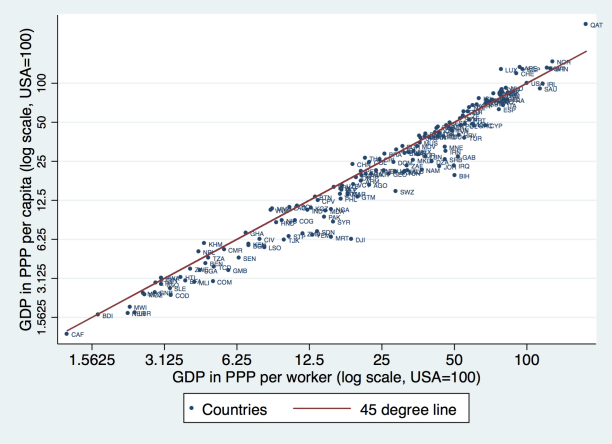
\includegraphics[width=5cm]{photos/gdp per capita.png} }}%
    \qquad
    \subfloat[\centering GDP per Worker]{{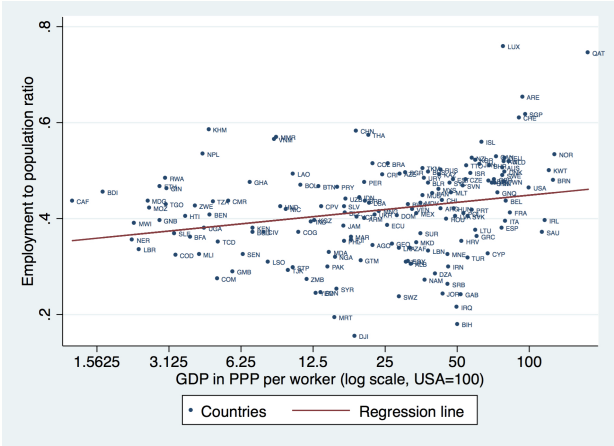
\includegraphics[width=5cm]{photos/gdp per worker.png} }}%
    \caption{Comparison of GDP in PP per capita and worker}%
    \label{fig:example}%
\end{figure}

We can see that relative GDP per capita is higher in rich countries mostly because the worker to population ratio is slightly higher in said countries.

\subsection{Convergence in GDP per capita across countries}

There was large divergence between countries from 1800 to 1950, but since then until 2000 it was quite stable \textit{on average} with some countries converging and others diverging.

\section{Accounting with Exogenous Physical and Human Capital}

\subsection{Production Function}

\begin{shaded}
    Assume that GDP(Y) is produced according to:
    \[Y=K^\alpha(ALh)^{1-\alpha}\]
    where:
    \begin{itemize}
        \item $k$ is the aggregate physical capital stock, $L$ is the number of workers, $h$ is the \textit{average} human capital per worker.
        \item $A$ is the \textbf{total factor productivity (TFP)}
        \item The parameter $\alpha \in (0,1)$ is the physical capital factor share.
    \end{itemize}
\end{shaded}

Dividing both sides by $L$ gives:
\begin{equation}
\label{gdppc}
    y = A^{1-\alpha} k^\alpha h^{1-\alpha}
\end{equation}

where $y \equiv \frac{Y}{L}$ and $k \equiv \frac{K}{L}$ are output and physical capital per worker.

\begin{shaded}
\textbf{\underline{Properties of this functional form}}
    \begin{itemize}
    \item \textbf{Diminishing Marginal Returns} to the three factors $K, L$ and $h$ $\Rightarrow$ more of any single factor raises $Y$, but the effect becomes smaller as the factor increases.
    \item \textbf{Constant returns to scale} in $K$ and $L$ $\Rightarrow$ Doubling $K$ and $L$ doubles $Y$.
\end{itemize}
\end{shaded}

We want to use Equation \eqref{gdppc} to see how much of the cross-time and cross-country variation in $y$ can be explained by factors $k$ and $h$.

\subsection{Measuring Physical Capital}
$K$ represents the total value of physical capital in the economy and it can be computed as:
\[K_t = I_{t-1} + (1-\delta)K_{t-1}\]
where $I$ represents investment and $\delta$ is the typical depreciation over the period. Because the level of investment $I$ is reported in the national accounts, we only need to know $K_0$ to construct the series. This is the \textit{perpetual inventory method.}

Growth theory suggests that $K_0 = \left( \dfrac{1}{g+\delta}\right) I_0$, where g is the growth rate of $K$. If 0 is sufficiently far in the past it will  not matter much because capital accumulated in time 0 will mostly be depreciated by time $t.$

\subsection{Measuring Average Human Capital}

Theory suggests that with competitive markets a worker earns $w \times h$, wage multiplied by the workers human capital. By comparing individuals with different schooling attainments \textit{in a given economy} (i.e. for a given $w$) one can infer the market value of human capital.
\subsubsection{Human capital as a function of schooling}

Assume that $h = e^{\phi(s)}$ where $\phi(\cdot)$ is a function of years of schooling in the economy $s$. The relationship between earnings and an extra year of schooling is log-linear suggesting:
\[\log h = \phi(s) = \text{constant} \times s\]
This is interpreted as: an extra year of schooling increases wage by a constant \% where the constant is obtained by micro data. In poorer countries where average schooling is low, a year of schooling procures larger gains than in rich countries.

\subsection{Accounting success of exogenous factors}

From the Cobb Douglas production function \eqref{gdppc}, we can define the "factor-only" model as:
\[y_{KH} \equiv k^\alpha h^{1-\alpha}\]
with
\begin{equation}
\label{factor only}
    y = A^{1-\alpha} y_{KH}
\end{equation}


We use $\alpha= 1/3$ because on average across the world and time physical capital earns about 1/3 of national income.
\subsubsection{Variance decomposition}
Taking logs of \eqref{factor only} gives:
\[\log y = (1-\alpha) \log A + \log y_{KH}\]
we have:
   
    \begin{align}
     \label{variance decomp}
    \begin{split}
        var\left[\log y\right] &= var\left[(1-\alpha) \log A + \log y_{KH}\right] \\
        &= var\left[ \log y_{KH} \right] + (1-\alpha)^2 var\left[ \log A\right] + 2(1-\alpha) cov\left[ \log y_{KH}, \log A \right]
    \end{split}
    \end{align}

    \begin{shaded}
        Define:
        \begin{equation}
        \label{success1}
            \text{success}_1 \equiv \dfrac{var\left[ \log y_{KH}\right]}{var\left[ \log y \right]}.
        \end{equation}
        

        How much of the empirical cross-time ot cross-country variation of $\log y$, is accounted for by the variation of the factor only model $\log y_{KH}$.
    \end{shaded}
        \begin{note}
        statistical notes:
        \begin{itemize}
            \item If $A$ is identical across observations, then $var\left[\log A\right] = 0$ and $cov\left[ \log y_{KH}, \log A \right]= 0$, implying that $\text{success}_1 = 1$.
            \item If $A$ varies across observationsm then $var \left[ \log A \right] >0$. If, in addition, $cov\left[ \log y_{KH}, \log A \right] \geq 0$ (meaning observations with more factors tend to have higher $A$), then $(1-\alpha)^2 var\left[ \log A\right] + 2(1-\alpha) cov\left[ \log y_{KH}, \log A \right]>0$, and therefore $\text{success}_1<1$
        \end{itemize}
        \end{note}
\subsubsection{Inter-percentile range}

To account for outliers we can measure the $90^{th}$ to $10^{th}$ percentile in terms of $y_{KH}$ and $y$.
\begin{equation}
    \label{success2}
    \text{success}_2 = \dfrac{\dfrac{y_{KH}^{90}}{y_{KH}^{10}}}{\dfrac{y^{90}}{y^{10}}}
\end{equation}

\begin{equation}
\begin{array}{c|cc|c||cc|c} 
& \operatorname{var}\left[\log y_{K H}\right] & \operatorname{var}[\log y] & \text { success }_1 & \frac{y_{K H}^{90}}{y_{K H}^{10}} & \frac{y^{90}}{y^{10}} & \text { success }_2 \\
\hline \text { US } & 0.03 & 0.14 & 0.31 & 1.66 & 2.48 & 0.67 \\
\text { UK } & 0.05 & 0.15 & 0.35 & 1.86 & 2.86 & 0.65 \\
\text { China } & 0.25 & 0.46 & 0.54 & 3.99 & 5.98 & 0.67 \\
\text { India } & 0.06 & 0.24 & 0.27 & 1.96 & 3.90 & 0.50 \\
\hline
\end{array}
\end{equation}

\begin{itemize}
    \item $\text{success}_1$ shows that about a third of GDP per worker across time can be "accounted for" by factor intensity
    \item$\text{success}_2 > \text{success}_1$ shows that according to this measure, factors "matter more".
\end{itemize}

\subsubsection{Improving the factor only model}

(Equation:\eqref{factor only})

Caselli (2005) considers many adjustments to the factor-only model which gives it more explanatory power. These improvements relate to improves quality-based measures of $h$ and $k$.
        
Alternative measures $h$ and $k$ that account for better quality differences:
\begin{enumerate}
    \item \textbf{Quality of schooling}: typically lower in poorer countries, meaning that our measure of $h$ is overestimated so an adjusted measure of $y_{KH}$ would have more explanatory power.
    \item \textbf{Experience}: Human capital also accumulates through work experience. In poorer countries workers on average have more work experience, but typically have lower returns from experience.
    \item \textbf{Health}: Workers in poorer countries are typically less healthy, which can impair physical and cognitive function and hence exaggerate our measure of $h$.
    \item \textbf{R\&D content of physical capital}: The quality $k$ is probably lower in poorer countries because of lower R\&D content. The magnitude of this effect is difficult to establish.
\end{enumerate}

\section{Solow Model}
\subsection*{Set Up}
\begin{shaded}
\begin{itemize}
    \item Time $t$ is discrete and runs from 0 to $\infty$, $t=\{1, 2, \ldots\}$.
    \item One representative agent (representative household and firm):
    \begin{itemize}
        \item owns all labour and capital in the economy; and
        \item makes all decisions
    \end{itemize}
    \item The law of motion. Mentioned in Section 2.2 is the following:
    \begin{equation}
        \label{capital stock}
        K_{t+1} = (1-\delta)K_t + I_t
    \end{equation}
    where initial capital $K_0>0$ is exogenous.
\end{itemize}
\end{shaded}

\subsubsection*{Household}

The household chooses the proportion of its income to invest from an exogenous fraction $s\in(0,1)$.
\begin{equation}
    \label{household invest}
    I_t = sY_t
\end{equation}

The remainder is consumed according to the resource constraint:
\begin{equation}
    \label{constraint}
    C_t + I_t = Y_t
\end{equation}

\subsubsection*{Production}
Output $Y$ is assumed Cobb-Douglas:
\begin{equation}
    \label{solow production}
    Y_t = K_t^\alpha(AL)^{1-\alpha}.
\end{equation}

\begin{note}
    In the simplest version of the Solow model we keep $L$ and $A$ constant. Additionally, we could use the production function used earlier which includes human capital $h$, but this does not add much to the analysis.
\end{note}

Substituting \eqref{solow production} and \eqref{household invest} in to \eqref{capital stock}, we have a new equation:
\begin{equation}
    K_{t+1} = (1-\delta)K_t + sK_t^\alpha(AL)^{1-\alpha}, \forall t = \{0,1,2,\ldots\}
\end{equation}
starting from some $K_0$. Once we know the series of $K_t$ we immediately know all other variables: $Y_t, I_t, C_t$.

\subsection{Dynamics of K}

\subsubsection{Condition for positive capital growth}
$K_{t+1} > K_t$.
\begin{equation}
    \label{capital growth}
\end{equation}
\begin{gather*}
     (1-\delta)K_t + sK_t^\alpha(AL)^{1-\alpha} > K_{t+1} \\
     \Leftrightarrow s(AL)^{1-\alpha} > \delta K_t^{1-\alpha} \\
     \Leftrightarrow K_t < AL\left( \dfrac{s}{\delta}\right)^{\frac{1}{1-\alpha}}
\end{gather*}

Therefore:
\begin{itemize}
    \item If $K_t < ...$, then K will grow from $t$ to $t+1$ 
    \item If $K_t > ...$, then K will fall from $t$ to $t+1$
\end{itemize}

\begin{note}
    Because production is increasing in capital, $K_{t+1}>K_t$ implies $Y_{t+1} > Y_t$ and vice versa.
\end{note}

\subsubsection{Steady State}
We are in steady state when $K_{t+1} = K_t$. From \eqref{capital growth} we get steady state capital denoted $^*$:
\begin{equation}
    \label{steady state}
    K^* = AL\left( \dfrac{s}{\delta}\right)^{\frac{1}{1-\alpha}}.
\end{equation}

Steady state GDP:
\begin{equation}
\label{steady state gdp}
\begin{aligned}
Y^{\star} & =K^{\star \alpha}(A L)^{1-\alpha} \\
& =\left(A L\left(\frac{s}{\delta}\right)^{\frac{1}{1-\alpha}}\right)^\alpha(A L)^{1-\alpha} \\
& =A L\left(\frac{s}{\delta}\right)^{\frac{\alpha}{1-\alpha}}
\end{aligned}
\end{equation}

\subsubsection{Convergence of $K$}

Starting from some $K_0<(>)K^*$, over time, $K_t$ converges monotonically from below (above) towards $K^*$.

\begin{proof}
We must show that $K_{t+1}>K_t \Rightarrow K_{t+2}>K_{t+1}$\\
If $K_{t+1}>K_t$ we have $(1-\delta)K_{t+1} > (1-\delta)K-t$ this gives:
\begin{gather*}
    (1-\delta)K_{t+1} + bK_{t+1}^\alpha > (1-\delta)K_{t} + bK_t^\alpha + bK_{t+1}^\alpha - bK_t^\alpha \\
    \Leftrightarrow \underbrace{K_{t+2}}_{=(1-\delta)K_{t+1} + bK_{t+1}^\alpha} > \underbrace{K_{t+1}}_{=(1-\delta)K_{t} + bK_t^\alpha} + b[K_{t+1}^\alpha - K_t^\alpha]
\end{gather*}
where $b \equiv s(AL)^{1-\alpha}$ and our last term $b[K_{t+1}^\alpha - K_t^\alpha]$ is strictly positive under $K_{t+1}>K_t$, then it must be that indeed $K_{t+2}>K_{t+1}.$
\end{proof}

\begin{itemize}
    \item If $K_0<K^{\star}$, then $K_0<K_1<K_2<\ldots<K_{\infty}=K^{\star}$.
    \item If $K_0>K^{\star}$, then $K_0>K_1>K_2>\ldots>K_{\infty}=K^{\star}$.
    \item If $K_0=K^{\star}$, then $K_0=K_1=K_2=\ldots=K_{\infty}=K^{\star}$.
\end{itemize}

From this it is obvious to see that starting from some $K_0<(>)K^*$, over time, the growth rate of capital, $g_t^K$, converges from above (below) towards 0.

\subsubsection{Convergence of $Y$}

Because production is increasing in Capital, given the convergence of physical capital it follows that 

\begin{itemize}
    \item If $K_0<K^{\star}$, then $Y_0<Y_1<Y_2<\ldots<Y_{\infty}=Y^{\star}$.
    \item If $K_0>K^{\star}$, then $Y_0>Y_1>Y_2>\ldots>Y_{\infty}=Y^{\star}$.
    \item If $K_0=K^{\star}$, then $Y_0=Y_1=Y_2>\ldots=Y_{\infty}=Y^{\star}$.
\end{itemize}

\subsubsection{Intuition}
Suppose $K_0<K^*$, the economy will grow over time, but at a lower and lower rate, and eventually converge to the steady state due to \textbf{decreasing marginal returns to} $K$.\\

$\frac{\partial Y(K)}{\partial K} = \alpha K^{\alpha-1}(AL)^{1-\alpha}$ decreases as $K$ increases.

\begin{itemize}
    \item The representative agent saves a constant fraction $s$ of income, and invests in new capital. More capital increases GDP, but each additional unit of $K$ has an increasingly small effect on $Y$ and therefore investment ($I = sY$). Eventually the additional new capital matches the depreciated capital.
\end{itemize}

\section{Inter-Temporal Optimisation and Capital Accumulation}

The representative household in the Solow model does not optimise anything as its savings rate is fixed and exogenous. We now look at the Ramsey model which models capital accumulation under infinite horizon inter-temporal optimisation where saving is endogenous.

\subsection{Household's Preferences}

The representative household is of size $L$ and its period utility function is:
\[U(C_t) = \dfrac{C_t^{1-\theta}-1}{1-\theta}\]
with $\theta>0$. In this function we have diminishing marginal utility. The function allows for precautionary saving. $\theta$ is the concavity of the function. This household is \textit{infinitely lived} and discounts time at the discount factor $\beta \in (0,1)$. This gives us the household's lifetime utility:
\begin{equation}
\label{household utility}
    \begin{aligned}
        U &= \sum_{t=1}^\infty \beta^t \dfrac{C_t^{1-\theta}-1}{1-\theta} \\
        &= \dfrac{C_0^{1-\theta}-1}{1-\theta} + \beta \dfrac{C_1^{1-\theta}-1}{1-\theta} + \beta^2 \dfrac{C_2^{1-\theta}-1}{1-\theta} + \beta^3 \dfrac{C_3^{1-\theta}-1}{1-\theta} + \cdots
    \end{aligned}
\end{equation}

\begin{note}
    The period utility function is strictly increasing and concave in $C$. Meaning the household always prefers more consumption, but the marginal utility decreases as $C$ rises. When $\theta=1$, the utility becomes $u(C_t) = \log C_t$
\end{note}

\begin{note}
    Because $\beta<1$ the household is \textbf{impatient}.
\end{note}

\subsection{Household's Budget Constraint}

Production function: 
\[Y_t = K_t^\alpha (AL)^{1-\alpha}\]

For $\forall t \geq 0$, the household budget constraint is:
\[C_t + \underbrace{K_{t+1}-(1-\delta)K_t}_{=I_t} = (1-\tau)K_t^\alpha(AL)^{1-\alpha} + T_t\]

RHS (Revenue/income):
\begin{itemize}
    \item Income from producing output is being taxed at rate $\tau$.
    \item Lump sum transfer $T-t$
\end{itemize}

LHS (Expenditure):
\begin{itemize}
    \item Consumption
    \item Investment/saving. Capital $K_{t+1}$ minus the un-depreciated current capital $(1-\delta)K_t$
\end{itemize}

\subsection{Types of Variables}

We have two types of variables: \textit{choice} and \textit{state} variables. In each period $t$, the household has two \textbf{choice variables}: $C_t$ and $K_{t+1}$. The household chooses these variables to maximise their utility subject to the budget constraint. That is:
\[\mathop{max}_{C_t, K_{t+1}} U = \sum_{t=1}^\infty \beta^t \dfrac{C_t^{1-\theta}-1}{1-\theta} \text { s.t. } C_t + K_{t+1} - (1-\delta)K_t = (1-\tau)K_t^\alpha(AL)^{1-\alpha} + T_t\]

The current capital stock $K_t$ is a \textbf{state variable} because it cannot be altered in time $t$.$T_t$ is another state variable.

\subsection{Economic Wedge}

In equilibrium, the lump sum transfer must equal the taxed revenue:
\[T_t = \tau K_t^\alpha(AL)^{1-\alpha}\]

Our main assumption is that the household does NOT internalise this relationship, they do not know that their direct transfers come from their taxed income. $\tau$ should not only be seen as a tax, but as a wedge that redistributes the return to economic activity. For example: corruption, expropriation, lack of contract enforcement, market power.

\subsection{Household's Problem}

As stated with the choice variables, the household is trying to maximise its utility subject to the budget constraint. This means that we can use a Lagrangain to find optimal $C_t$ and $K_{t+1}$.

\begin{shaded}
    \begin{equation}
\label{lagrange}
    \mathcal{L} = \sum_{t=0}^\infty \beta^t \dfrac{C_t^{1-\theta}-1}{1-\theta} + \sum_{t=0}^\infty \lambda_t \left[ (1-\tau)K_{t}^{\alpha}(AL)^{1-\alpha} + T_t - C_t - K_{t+1} - (1-\delta)K_t\right]
\end{equation}
\end{shaded}


By writing out the Lagrangian to $t=2$:
\begin{equation}
\begin{aligned}
\mathcal{L}= & \max _{\left\{C_t, K_{t+1}\right\}_{t=0}^{\infty}}\left\{\frac{C_0^{1-\theta}-1}{1-\theta}+\beta \frac{C_1^{1-\theta}-1}{1-\theta}+\beta^2 \frac{C_2^{1-\theta}-1}{1-\theta}+\ldots\right. \\
& +\lambda_0\left[(1-\tau) K_0^\alpha(A L)^{1-\alpha}+T_0-C_0-K_1+(1-\delta) K_0\right] \\
& +\lambda_1\left[(1-\tau) K_1^\alpha(A L)^{1-\alpha}+T_1-C_1-K_2+(1-\delta) K_1\right] \\
& \left.+\lambda_2\left[(1-\tau) K_2^\alpha(A L)^{1-\alpha}+T_2-C_2-K_3+(1-\delta) K_2\right]+\ldots\right\}
\end{aligned}
\end{equation}

\begin{note}
    There are an infinite number of terms. Also we can see that each consumption term appears twice, while each capital term appears three times.
\end{note}

\begin{shaded}
    By finding the FOC w.r.t. $C_t$ we get $\beta^t (1-\theta)\frac{C_t^{-\theta}}{1-\theta} -\lambda_t= 0$ or:
    \begin{equation}
    \label{foc ct}
        \beta^t C_t ^{-\theta} = \lambda_t
    \end{equation}
Finding the FOC w.r.t $K_{t+1}$ we get:
\begin{equation}
\label{foc kt1}
    \lambda_{t+1}\left[(1-\tau)\alpha K_{t+1}^{\alpha-1}(AL)^{1-\alpha} + 1-\delta \right] = \lambda_t
\end{equation}
\end{shaded}

Using \eqref{foc ct} for periods $t, t+1$ and substituting in to \eqref{foc kt1} we get:

\begin{equation*}
\begin{aligned}
& \Leftrightarrow \beta^t C_t^{-\theta}=\beta^{t+1} C_{t+1}^{-\theta}\left[(1-\tau) \alpha K_{t+1}^{\alpha-1}(A L)^{1-\alpha}+1-\delta\right] \\
& \Leftrightarrow C_{t+1}^\theta C_t^{-\theta}=\beta\left[(1-\tau) \alpha K_{t+1}^{\alpha-1}(A L)^{1-\alpha}+1-\delta\right]
\end{aligned}
\end{equation*}
Or more elegantly, we have

\begin{shaded}
The \textbf{Euler Equation}
    \begin{equation}
    \label{euler}
\left(\frac{C_{t+1}}{C_t}\right)^\theta=\beta\left[1+(1-\tau) \alpha K_{t+1}^{\alpha-1}(A L)^{1-\alpha}-\delta\right] .
\end{equation}

The Euler equation guides behaviour, namely the inter-temporal substitution of consumption. 
\begin{intu}
\[\left(\frac{C_{t+1}}{C_t}\right)^\theta=\beta\left[1+\underbrace{(1-\tau) \alpha K_{t+1}^{\alpha-1}(A L)^{1-\alpha}-\delta}_{\text { tomorrow's net return of investment } r_{t+1} = (1-\tau)R_{t+1} - \delta}\right] \]

A low rate of return induces the house hold to decrease consumption tomorrow relative to today. $\theta$ determines how much the household values consumption smoothing. A low $\theta$ implies the household reacts strongly to the relative rate of return (i.e. less smooth consumption)




\end{intu}

\end{shaded}

Example with $\beta = 0.95$
\begin{equation}
\begin{array}{c|c|c|c} 
& r_{t+1}=0 & r_{t+1}=\frac{1}{\beta}-1 \approx .05 & r_{t+1}=0.2 \\
\hline \theta=0.33 & 0.86 & 1 & 1.49 \\
\theta=1 & 0.95 & 1 & 1.14 \\
\theta=3 & 0.98 & 1 & 1.04
\end{array}
\end{equation}

We can see when the rate of return is 0 and $\theta = 0$, $\dfrac{C_{t+1}}{C_t}=0.86$, meaning we will consume less  tomorrow. 

\begin{intu}
    Intuitively this is because the household is reactionary to the relative rate of return and seeing as it is 0, there is no need to save. However, when $\theta=3$ we consume almost exactly the same amount as today (0.98).

When the discount rate is exactly equal to the rate of return, consumption today and tomorrow will equate.

When the net rate of return (rate of return minus discount) is positive we will save and consume more tomorrow. And we see again that a low $\theta$ means that we will save more when rate of return is higher relative to a higher $\theta$.
\end{intu}


The Euler equation tells us the path of consumption not the level of consumption.

\subsubsection{Resource Constraint}

The Euler equation indicates what the household \textit{wants} to do. The budget constraint tells us what the household \textit{can} do.
\begin{equation}
    \label{budget constraint}
    C_t + K_{t+1} - (1-\delta)K_t = (1-\tau)K_t^\alpha (AL)^{1-\alpha} + T_t
\end{equation}

We assume that the "taxed" income is returned back to the household, so we have $T_t = \tau K_t^\alpha(AL)^{1-\alpha}$

\subsection{Equilibrium}

Because of this assumption about "tax" we know that \textbf{in equilibrium} the household's budget constraint is:
\begin{equation}
    \label{eq budget constraint}
    C_t + K_{t+1} - (1-\delta)K_t = K_t^\alpha(AL)^{1-\alpha}
\end{equation}

\begin{note}
    The reason that Equation \eqref{budget constraint} and Equation \eqref{eq budget constraint} are different, is because we need to ensure that the household is unaware of the link between $\tau$ and $T$. The household perfectly predicts the value of $T$, but we do not want the household to understand that if it invests more into $K$ this will lead to a higher $T$.
\end{note}

\begin{shaded}
    The equilibrium is a set of variables $\{C_t, K_{t+1}\}_{t=0}^\infty$ s.t. the Euler Equation \eqref{euler} and the resource condition \eqref{eq budget constraint} are satisfied $\forall t = 0,1,2,\ldots$. That is both equations:
    \[\left(\frac{C_{t+1}}{C_t}\right)^\theta=\beta\left[1+(1-\tau) \alpha K_{t+1}^{\alpha-1}(A L)^{1-\alpha}-\delta\right]\]
    and
    \[C_t + K_{t+1} - (1-\delta)K_t = K_t^\alpha(AL)^{1-\alpha}\]
    are satisfied.
    \begin{note}
        The initial $K_0$ is exogenously given, therefore not a variable.
    \end{note}
\end{shaded}

\subsubsection{Solving for the equilibrium}

Because we have an infinite time horizon to solve for the values of the variables, we would have to do an infinite number of equations simultaneously. We can see this from expressing the two equations in time $t=0,1$.

\begin{equation}
\begin{gathered}
C_0+K_1-(1-\delta) K_0=K_0^\alpha(A L)^{1-\alpha}, \\
\left(\frac{C_1}{C_0}\right)^\theta=\beta\left[1+(1-\tau) \alpha K_1^{\alpha-1}(A L)^{1-\alpha}-\delta\right], \\
C_1+K_2-(1-\delta) K_1=K_1^\alpha(A L)^{1-\alpha}, \\
\left(\frac{C_2}{C_1}\right)^\theta=\beta\left[1+(1-\tau) \alpha K_2^{\alpha-1}(A L)^{1-\alpha}-\delta\right] .
\end{gathered}
\end{equation}

In the first equation, we have two unknown variables ($C_0, L_{t+1}$), which implies we need one more equation to solve them simultaneously. However, this second equation brings in another unknown variable $C_1$, so we need another equation to solve simultaneously. and so on \ldots.

\subsection{Steady State}

Just as in the Solow Model, the Ramsey model converges to a steady state s.t. $K_t = K_{t+1} = K^*, C_t = C_{t+1} = C^*$ which implies $Y_t = Y_{t+1} = Y^*$

\begin{shaded}
    The Euler equation \eqref{euler} and the resource constraint \eqref{eq budget constraint} in steady state are as follows:

    \begin{equation}
        \label{ss euler}
        1 = \beta\left[1 + (1-\tau) \alpha K^{*\alpha-1} (AL)^{1-\alpha} - \delta \right]
    \end{equation}
    \begin{equation}
        \label{ss budget constraint}
        C^* + K^* - (1-\delta)K^* = K^{*\alpha} (AL)^{1-\alpha}
    \end{equation}
\end{shaded}

\subsubsection{Steady State Capital}

Using the steady state euler equation \eqref{ss euler}, we can solve for the steady state level of capital, $K^*$:
\begin{equation}
\begin{array}{r}
\frac{1}{\beta}=1+(1-\tau) \alpha K^{\star \alpha-1}(A L)^{1-\alpha}-\delta \\
\Leftrightarrow \frac{1-\beta(1-\delta)}{\beta}=(1-\tau) \alpha K^{\star \alpha-1}(A L)^{1-\alpha} \\
\Leftrightarrow K^{\star 1-\alpha}=\frac{\beta(1-\tau) \alpha(A L)^{1-\alpha}}{1-\beta(1-\delta)}
\end{array}
\end{equation}

which gives us:
\begin{mdframed}
    \begin{equation}
\label{ss capital}
K^{\star}=\left(\frac{\beta(1-\tau) \alpha}{1-\beta(1-\delta)}\right)^{\frac{1}{1-\alpha}} A L
\end{equation}
\end{mdframed}

\subsubsection{Steady State Consumption}

Now that we have steady state capital we can substitute it in to the steady state resource constraint equation \eqref{ss budget constraint} to find $C^*$:

\begin{mdframed}
    \begin{equation}
        \label{ss consumption}
        C^* = \left(\dfrac{\beta(1-\tau)\alpha}{1-\beta(1-\delta)}\right)^{\dfrac{\alpha}{1-\alpha}}AL-\delta\left(\dfrac{\beta(1-\tau)\alpha}{1-\beta(1-\delta)}\right)^{\dfrac{1}{1-\alpha}}AL
    \end{equation}
\end{mdframed}

\subsubsection{Steady State GDP}
We knpw that the Steady State GDP equation is simply $Y^* = K^{*\alpha}(AL)^{1-\alpha}$. So by substituting our equation \eqref{ss capital} in to this we get:

\begin{mdframed}
    \begin{equation}
        \label{ss gdp}
        Y^* =\left(\frac{\beta(1-\tau) \alpha}{1-\beta(1-\delta)}\right)^{\frac{\alpha}{1-\alpha}} A L 
    \end{equation}
\end{mdframed}

\subsubsection{Comparative Statistics}

Our key steady-state equations are \eqref{ss capital} and \eqref{ss gdp}. We must look at the relationship between each of these steady-state variables and the parameters.

\begin{itemize}
    \item $\nearrow \beta \Rightarrow \nearrow K^*, \nearrow Y^*$

    \begin{intu}
        More patient households save more and accumulate more capital (i.e. the equilibrium rate of return is lower when households are more patient)
    \end{intu}
    \item $\nearrow \tau \Rightarrow \searrow K^*, \searrow Y^*$

    \begin{intu}
        A higher "tax"/economic wedge disincentives investment because the household does NOT perceive the full return
    \end{intu}
\end{itemize}

\begin{note}
    The steady state capital per worker $\frac{K^*}{L}$ and GDP per worker $\frac{Y^*}{L}$ do \textit{NOT} depend on the number of workers.
\end{note}

\subsection{Dynamics outside of the Steady State}

In general, the Ramsey model is similar to the Solow Model:
\begin{itemize}
    \item If $K_0 < K^*$, then $K$ and $Y \nearrow$ and eventually reach $K^*$ and $Y^*$.
    \item If $K_) > K^*$, then $K$ and $Y \searrow$ and eventually reach $K^*$ and $Y^*$.
\end{itemize}
\begin{shaded}
    \subsection*{Main Differences between Solow and Ramsey Models}

    \begin{itemize}
        \item \textbf{Speed of convergence}. Because the household now adjusts the implied savings rate $s_t = \frac{I_t}{Y_t}$ as time goes by.

        \item \textbf{The reaction to anticipated changes in the economic environment}. (not convered here)
    \end{itemize}
\end{shaded}

\newpage

\subsubsection{Numerical example of Convergence}

\begin{figure}[h]
    \centering
    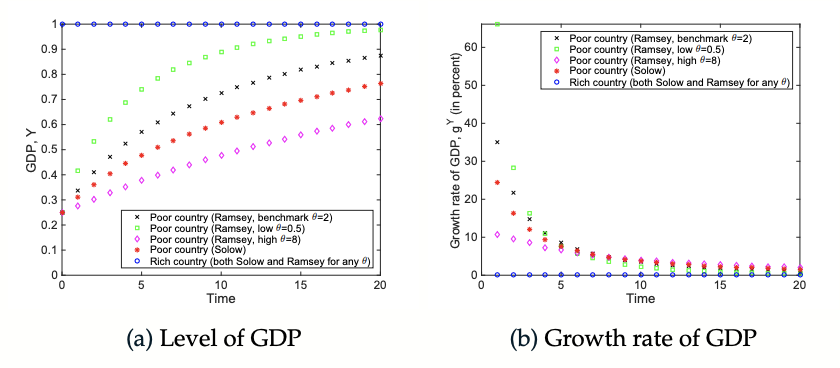
\includegraphics[width=15cm]{photos/example of convergence.png}
    \caption{Illustration of convergence}
    \label{fig:convergence}
\end{figure}

Above we see in the first period the growth rate of GDP, due to high build-up of capital, with $\theta=2$ is about 35\% per year. Thus convergence to steady state is likely to be even faster than in Solow.

\begin{note}
    Empirical estimates give a range for $\theta$, but typically centers on $\theta\approx2$. 
\end{note}

\paragraph{Numerical example comment}

Given the speed of the convergence, the Ramsey model suggests that large income differences across economies (e.g. US vs China today, or US today vs US 50 years ago) are unlikely to be the result of differences in $K$ only, because they are undone within a few years.

Close to steady state, the Ramsey model offers insights into why economies sometimes grow relatively fast (booms) and sometimes relatively slow (recessions).

\subsection{Extending the model}

We can include growth rates for both technology and population s.t.:
\[L_t = L_0(1+n)^t\]
and 
\[A_t = A_)(1+g)^t.\]

When the population and technology grow, we find our economy on a growth path rather than in a steady state, i.e. consumption grows at a constant rate.

\begin{note}
    In this case again like the Solow Model, long term growth in GDP per worker equals the rate of technological progress $g$.
\end{note}

\subsection{Capital Output Ratio}

Capital output ratio can be defined as $\frac{K}{Y}$, and in steady state using equations \eqref{ss capital} and \eqref{ss gdp} we have a Steady State capital output ratio of:
\begin{equation}
\label{ss capital output ratio}
\begin{aligned}
\frac{K^{\star}}{Y^{\star}} & =\frac{\left(\frac{\beta(1-\tau) \alpha}{1-\beta(1-\delta)}\right)^{\frac{1}{1-\alpha}} A L}{\left(\frac{\beta(1-\tau) \alpha}{1-\beta(1-\delta)}\right)^{\frac{\alpha}{1-\alpha}} A L}=\left(\frac{\beta(1-\tau) \alpha}{1-\beta(1-\delta)}\right)^{\frac{1-\alpha}{1-\alpha}} \\
& =\frac{\beta(1-\tau) \alpha}{1-\beta(1-\delta)}
\end{aligned}
\end{equation}

\begin{note}
    This steady state capital output ratio is independent of $A$
\end{note}

We can link it to preference and institutional parameters:
\begin{itemize}
    \item $\frac{K^*}{Y^*}$ is increasing in $\beta \Rightarrow$ more patient households have higher $\frac{K^*}{Y^*}$
    \item $\frac{K^*}{Y^*}$ is decreasing in $\tau \Rightarrow$ more distorted economies have lower $\frac{K^*}{Y^*}$.
\end{itemize}

Suppose poor economies are inefficient because of two underlying reasons: 1) low total factor productivity, $A$. 2) High distortions to economic activity $\tau$. Then output will be low for two reasons: 1) directly through the low $A$ and 2) through low $K$, which is itself a result of low $A$ and high $\tau$.

The capital ourput ratio isolates the effect of $\tau$ of $K$ and is not contaminated by low $A$.

\subsection{Alternative factor-only model}

By reinterpreting the $A$ in our model $Y= K^\alpha(AL)^{1-\alpha}$ and we interpret it as being both total factor production $A$ and human capital $h$ we have: $Y = K^\alpha(ALh)^{1-\alpha}$ as in Section 2, along with the equation for gdp per capital \eqref{gdppc}:
\[y = A^{1\alpha}k^\alpha h^{1-\alpha}\]

We can manipulate this equation and multiply each side by $y^{-\alpha}$:
\begin{align*}
    y &= A^{1\alpha}k^\alpha h^{1-\alpha} \\
    y^{1-\alpha} &= A^{1-\alpha}k^\alpha h^{1-\alpha}y^{-\alpha} \\
    y^{1-\alpha} &= A^{1-\alpha} \left(\dfrac{k}{y}\right)^\alpha h^{1-\alpha} \\
    y &= A \left(\dfrac{k}{y}\right)^{\dfrac{\alpha}{1-\alpha}}
\end{align*}

\begin{mdframed}
Now we create an alternative "factor-only" model

\begin{equation}
    \label{alt factor only}
    y_{KH} = \left(\dfrac{k}{y}\right)^{\dfrac{\alpha}{1-\alpha}}
\end{equation}
\end{mdframed}

The reason for this alternative factor-only model is because our theory (both Ramsey and Solow) implies that $k$ not only causes $y$, but that in fact in the long term, both $k$ and $y$ are driven by $A$.

The capital output ratio $\frac{k}{y}$ is possibly a more adequate explanatory variable as it is independent of $A$. Therefore, by using it instead of $k$, we capture better the relative capital intensity of the economy.
\begin{intu}
    This can be thought of as deriving from sources such as investment distortions, $\tau$, or preferences for saving, $\beta$.
\end{intu}

\subsubsection{Comparing success between factor-only models}

By using the metrics of success established in Section 2.4 Equations \eqref{success1} and \eqref{success2} we can tabulate thr different metric of success between countries and time AND between models.

\begin{equation}
\begin{aligned}
&\begin{array}{c|cc|cc} 
& \multicolumn{2}{|c}{y_{K H}=\left(\frac{k}{y}\right)^{\frac{\alpha}{1-\alpha}} h} & \multicolumn{2}{c}{y_{K H}=k^\alpha h^{1-\alpha}} \\
& \text { success }_1 & \text { success }_2 & \text { success }_1 & \text { success }_2 \\
\hline \text { US } & 0.12 & 0.54 & 0.31 & 0.67 \\
\text { UK } & 0.16 & 0.52 & 0.35 & 0.65 \\
\text { China } & 0.39 & 0.58 & 0.54 & 0.67 \\
\text { India } & 0.09 & 0.37 & 0.27 & 0.50 \\
\hline
\end{array}\\
&\begin{array}{c|cc|cc} 
& \multicolumn{2}{|c}{y_{k h}=\left(\frac{k}{y}\right)^{\frac{\alpha}{1-\alpha}} h} & \multicolumn{2}{c}{y_{k h}=k^\alpha h^{1-\alpha}} \\
& \text { success }_1 & \text { success }_2 & \text { success }_1 & \text { success }_2 \\
\hline 2014 & 0.12 & 0.12 & 0.28 & 0.23 \\
1984 & 0.26 & 0.22 & 0.39 & 0.35 \\
1954 & 0.30 & 0.42 & 0.43 & 0.44 \\
\hline
\end{array}
\end{aligned}
\end{equation}

We see that for any comparison, the accounting success is lower with the alternative model than the original factor-only model. Some of the variation is accounted for by $h$ and $\frac{k}{y}$ but ultimately mostly due to something else, $A$. This suggests that productivity, $A$, is even more important in understanding GDP.

\subsection{Simple Ramsey Model}

What have we learnt?
\begin{shaded}
    \begin{itemize}
        \item Similar to the Solow Model, intertemporal optimization leads to a steady state of 0 long run GDP growth.
        \begin{itemize}
            \item This occurs even when households actively decide how much to save/invest
            \item The main driving force for this is that the production function is assumed to have diminishing marginal returns to capital.
        \end{itemize}
        \item The analysis is richer from the Ramsey model because investment decisions depend on preference parameters ($\beta, \theta$) and policy parameters ($\tau$).
        \begin{itemize}
            \item Outside of steady state, these parameters determine the speed of convergence.
            \item In stead state, they provide a deeper understsnding for why some economies have \textit{relatively} more physical capital (higher capital output ratio) than others.
        \end{itemize}
        \item The alternative factor-only model helps us revisit the question of how much the factors $\frac{k}{y}$ and $h$ contribute to variations in GDP. 
        \begin{itemize}
            \item We concluded that TFP plays an even larger role in determining GDP than expected.
        \end{itemize}
    \end{itemize}
\end{shaded}

\section{Total Factor Productivity}

We have found that Total Factor Productivity (TFP), $A$, is crucial for explaining variations in GDP per worker across time and space. It is important when recovered as residual after accounting for contribution of exogenous $K$ and $H$. Additionally, it is imoirtant after taking into account that variation in $K$ is endogenous and to a large extent determined by $A$. So, we must figure out what $A$ is.

\subsection{Production}

Instead of our production function assumption $Y = A^{1-\alpha} \times K^\alpha H^{1-\alpha}$, we will consider an alternative specification of the form:
\[Y = A \times F(K,H,Q)\]
where $F$ is a function of $K,H,Q$.

We assume that $K,H,Q$ are \textbf{rivalrous }production factors, while $A$ is a catch-all for \textbf{non-rivalrous} production factors.

\subsubsection{Rivalrous Production Factors}
Definition: if one person (or firm, or economy) uses it, another one cannot use it at the same time. Prime example: physical and human capital $K,H$.

Because economies are generally geographic entities, the easiest way to think of $Q$ is as land, both quality and quantity.
\begin{itemize}
    \item This can be quality of soil, natural resources like minerals, water, or can be things like connectivity to other economies, topography and natural amenities.
\end{itemize}

The function $F$ is constant returns to scale with respect to all its arguments. e.g. Cobb-Douglas:
\[F(KH,Q) = Q^\gamma K^\alpha H ^{1-\alpha-\gamma}\]
with $\alpha + \gamma <1$

\begin{intu}
    Holding $A$ fixed, one could in theory replicate the UK economy by doubling its $K,H,Q$.
\end{intu}

With the previous assumption we have:
\begin{equation}
    \label{Y QKH}
    Y = \underbrace{A Q^\gamma}_{TFP} K^\alpha H^{1-\alpha-\gamma}
\end{equation}
In practice lots of research sets $\gamma=0$.

\subsubsection{Non-Rivalrous Factors, $A$}

Definition: If one person (or firm, or economy) uses it, this does NOT preclude anyone else from using it.

Things like ideas, also referred to as knowledge, technology, blueprints or recipes etc.

Ideas enhance output through \textbf{product innovation} (generating new products/varieties), or \textbf{process innovation} (improving the production process, cutting the cost of production, of existing products).

Examples: kindling fire, calculus, formula for aspirin, idea of conveyor belt, idea of just-in-time inventory.

\subsubsection{Example}
Nuclear power:
\begin{itemize}
    \item The technology/idea of how to extract nuclear power is codified in a book or computer program: $A$
    \item The engineers that understand and can apply the knowledge: $H$
    \item The equipment in the power plant: $K$.
\end{itemize}

\subsection{Decomposition of Ideas/Technology}

COnsider a further decomposition for economy $j$ at time $t$
\[A_{j,t} = X_t \times E_{j,t}\]
where
\begin{itemize}
    \item $X$ is the stock of ideas available in the world at t particular time $\Rightarrow$ \textbf{World Technology Frontier}
    \item $E \in [0,1]$ is the efficiency at which these ideas are combined with production factors in a particular economy $\Rightarrow$ inverse of the \textbf{distance to the frontier.}
\end{itemize}

\subsubsection*{Growth vs Levels}

$X$ is the source for long-run \textbf{growth} in the world and common across countries.
\begin{itemize}
    \item [$\Rightarrow$]  without technological progress there can be no long-run growth
\end{itemize}


$E$ is stationary (steady or fluctuating) over time and represents country-specific \textbf{level}.
\begin{itemize}
    \item [$\Rightarrow$]  without variation of $E$, all countries make the same use of technology.
\end{itemize}

\subsection{Sources of Growth in the frontier, X}
We have three sources:
\begin{enumerate}
    \item Purely exogenous
    \item Externality
    \item Investment
\end{enumerate}

\newpage

\subsubsection{Ideas due to externalities}

There are several channels through which ideas can be created as spillovers. Prominent ones are:
\begin{enumerate}
    \item Economic activity and learning-by-doing
    \begin{itemize}
        \item As individuals/firms produce, they generate new ideas
    \end{itemize}
    \item Accumulation of human capital
    \begin{itemize}
        \item We can assume that human capital generates more/better ideas so spillovers are more likely when individuals are skilled
    \end{itemize}
    \item Interaction between people
    \begin{itemize}
        \item There are stronger spillovers when people individuals interact. 
    \end{itemize}
\end{enumerate}
In each case, a larger population leads to more spillovers.

\subsubsection{Ideas due to investment}

Assumption: the creation of any idea requires investment i.e. R\&D. 

The two possibilities that we have are:
\begin{enumerate}
    \item The idea is \textbf{non-excludable}. Once it exists, there is no possibility of excluding users.
    \begin{itemize}
        \item nonexcludability + non-rivalry = public goods
        \item In this case, individuals or firms have no monetary incentive to generate ideas, so it typically must be generated by governments
        \item example: basic research, typically done via public funding.
    \end{itemize}
    \item The idea is \textbf{excludable}. Once it exists, there are mechanisms to exclude users and sell the right to access the idea.
    \begin{itemize}
        \item either because the idea can be kept secret, or done through patents and intellectual property rights.
        \item Examples: pharmaceuticals, software, aviation, bio engineering.
    \end{itemize}
\end{enumerate}

\subsubsection{Main trade-off of investment in ideas:}

the economic trade offs associated with the creation of non-rivalrous  but (partially) excludable ideas is the main focus of modern \textit{Endogenous Growth Theory} \cite{romer1990}.

The main insight is long-term growth is only possible with excludability, which requires monopoly power, so some excludability is optimal, but not too much because $\ldots$
\begin{itemize}
    \item excludability also implies that ideas are not fully used (because the innovating firm has monopoly power);
    \item but also because the prospect of monopoly rents can lead to \textit{excessive} innovation due to business-stealing motive.
\end{itemize}

\subsubsection{How are ideas generated?}
Romer \cite{romer1990} suggests that ideas have a production function
\[A = f(\text{researchers, discovery rate of ideas, congestion})\]
where we have high fixed costs, and low marginal costs. The idea is only produced if the firm can charge more than the marginal cost $\rightarrow$ need some excludability.

\subsubsection{Market size}
Marlet size can help improve the production of ideas. The larger the market to which ideas can be sold, the more profitable the innovation. This can be large population or high income.

This implies that the growth rate of the technology frontier is positively affected by:
\begin{itemize}
    \item population size
    \item trade and globalisation that generate a larger market.
\end{itemize}


\subsubsection{Growth of population and technology}
We are interested in the two-way connection between population and output per capita.

Effect of population on output per capita:
\begin{itemize}
    \item $\nearrow$ because population growth leads to technological innovation.
    \item $\searrow$ because natural resources ($Q$) are largely in fixed supply so there are fewer resources per worker.
\end{itemize}

In addition output per capita is likely to affect population growth:
\begin{itemize}
    \item $\nearrow$ through Malthusian effect because individuals can afford to have more children.
    \item $\searrow$ because the opportunity cost of caring for children is higher when wages are high.
\end{itemize}

\subsubsection{Endogenous growth and Malthusian phase}

The unified growth theory explains:
\begin{enumerate}
    \item Malthusian era from 1 million BCE until about 1800 where population grew very slowly but output per capita stagnates
    \item post-Malthusian era from about 1800 until about mid-20th century where both population and output per capita growth increase.
    \item Modern growth era where population growth rate slows while output per capita growth continues.
\end{enumerate}

\subsection{Sources of Differences in Efficiency, E}

Given the world frontier of knowledge $X_t$, the production function $F(K,H,Q)$, and given an economy's rivalrous production factors $(K,H,Q)$, let \textbf{efficiency} be the residual:
\[E = \dfrac{Y}{X\times F(K,H,Q)}\]

Why may countries differ in how efficiently they use the existing frontier of knowledge? Maybe slow adoption of technology or mis-allocation.

\subsubsection{Why slow adoption of technology?}

The speed of idea diffusion is itself an externality. Areas that are not well-connected will learn less quickly.

Codified ideas must be implemented which often requires particular forms of human capital such as engineers or computer scientists.

Frontier technologies are typically developed in rich countries and adapted to their requirements, but they may be inefficient in developing countries. Example: high-yielding varieties of maize or wheat developed for temperate climates are less useful in tropics.

Government policies may block the spread of ideas.

BUT, as adoption of technologies speeds up over time, it is difficult to argue that poor countries have low TFP primarily because frontier technology has not reached them yet.

\subsubsection{What is mis-allocation?}

Mis-allocation implies that an economy could increase output bu re-allocating its aggregate stock of production factors. Too many resources allocated to low productivity firms/sectors/geographic areas and vice versa.

Efficient organisation is another form of a non-rivalrous technology.

\subsubsection{Misallocation in our model}
Example with our model:
\begin{mdframed}
    With an economy with 2 sectors, and total labour force $L$, labour employed in the 2 sectors is combined as follows
    \[L_Y = L_1^\sigma L_2^{1-\sigma}, \qquad Y = K^\alpha L_Y^{1-\alpha}\]
    If a share of workers $s$ work in sector 1, then $L_1 = sL, L_2 = (1-s)L$
    \[L_Y = (sL)^\sigma((1-s)L)^{1-\sigma} \Rightarrow Y = K^\alpha (s^\sigma (1-s)^{1-\sigma}L)^{1-\alpha}\]

    $s^\sigma (1-s)^{1-\sigma}$ can be thought of as labour-augmenting productivity. We can find FOC of $Y$ with respect to $s$. This gives us that the value of $s$ that will lead to the most production is , $s=\sigma$
\end{mdframed}

From the example we see that misallocation occurs when $s\neq\sigma$. If this is the case, then the economy will produce less than it could.

\subsubsection{Across firms}

in any economy there is a wide range of the productivity level between firms. Large gains in aggregate efficiency by reallocating resources from low-productivity firms to high-productivity firms.

\paragraph{Misallocation quantified} \mbox{} \\

Hsieh and Klenow (2005) \cite{hsieh2009} measured the dispersion of productivity in manufacturing is higher in India than in China and higher in China than in the US.

They interpret the difference in the dispersion between India or China relative to the US to be due to policies creating "wedges" (implicitly taxing some firms and subsidizing others). Reducing these wedges to the level of the US would increase TFP in India (China) by 50 (40) percent.

\subsubsection{Across sectors}

\begin{enumerate}
    \item \textbf{Agriculture}. Compared to rich countries ,poor countries have much lower labour productivity in agriculture relative to non-agriculture. However, poor countries have substantially higher employment in agriculture.

    \item \textbf{Sectors shielded from international trade}. Lowering barriers to international trade implies that economies can reallocate resources toward sectors in which they have a comparative advantage
\end{enumerate}

\subsubsection{Across Space}

The large productivity differences across countries suggest massive international misallocation of labour. Empirical studies have estimated that removing all restrictions to migration around the world would lead to an increae in welfare of more than 300\%.

Within countries too regions often vary immensely in productivity. Research in urban economies suggests that thee exists misallocation of labour across cities, with inefficiently many workers "stuck" in low-productive cities.
\begin{shaded}
    \subsubsection{Proximate Reasons for misallocation}
    \begin{itemize}
    \item Financial Frictions. Lack of credit implies that resources are disproportionately employed by wealthy and incumbent individuals/firms at the expense of entering and asset poor individuals/firms.

    \item Market Power. Monopolies maximise revenue by maintaining high prices which restricts their output, and hence their employment resources.

    \item Labour Market Frictions. Firing/hiring frictions slow down the reallocation of labour toward more productive firms.

    \item Tax policies/bribes. When some firms avoid taxes legally or illegally, these firms employ inefficiently many resources at the expense of other firms.

    \item Lack of Public Goods and Services. in sectors where markets function inefficiently (public goods, or sectors with information asymmetries i.e. health), an efficient allocation of resources requires public involvement.
\end{itemize}
\end{shaded}

\begin{mdframed}
    \begin{note}
    Even though misallocation lowers current output, it may be the case that it is not sub-optimal. This depends on the individual and how much weight they attach to objectives they pursue.

    Moving locations is costly as people are attached to their place of origin, and most productive locations feature low amenities (pollution, congestion, crime)

    Barriers to international trade can be justified on the grounds of national pride and self-sufficiency.

    Mechanisms that create inefficiency to current output, may potentially be \textit{dynamically efficient}
\end{note}
\end{mdframed}


\subsection{Fundamental determinants of X and E}

We will look at three possible distinctions of fundamental determinants for the two factors:
\begin{enumerate}
    \item Geography
    \item Culture
    \item Institutions
\end{enumerate}

\subsubsection{Geography}

There are many ways that geography can foster/prevent economic activities and ideas i.e. suitability of agriculture, disease environment, connectivity, and abundance of natural resources. 

Geography can set the scene for particular social and organisational patterns.

\subsubsection{Culture}
\textbf{Preferences:} relative importance that individuals attach to consumption, leisure, insurance, altruism, innovation etc.

\textbf{Beliefs:} extent to which individuals can coordinate on outcomes, trust each other and generally cooperate.

These two concepts matter for economic outcomes and the types of ideas that are produced and used.

\subsubsection{Institutions}

Institutions are/do two things:
\begin{enumerate}
    \item Humanly devised so that society can (collectively or individually) change the "rules of the game".

    \item Impose constraints and rewards for human behaviour. Policies, regulations and laws that punish certain behaviours and reward others.
\end{enumerate}

There are two types of institutions that we are interested in:
\begin{enumerate}
    \item Economic institutions. Implement rules that impact the structure of markets, the set of feasible contracts and transactions, redistribution etc.

    \item Political institutions. Implement rules underlying the process of collective decision-making, determining which economic institutions prevail.
\end{enumerate}

Nowadays, the institutional hypothesis is arguably the most influential fundamental explanation for long-run economic performance, but not the sole reason.

Inferior equilibria persist because they may benefit certain segments of society (often called \textit{elite capture})

\subsubsection{Difficulty in distinguishing causes}

It is difficult and unethical to run experiments, and difficult to measure the quality of institutions.

There may be reverse causality (can richer countries afford better institutions?). Endogeneity and omitted variables may affect wealth and culture/institutions.

\begin{mdframed}
    

\paragraph{Becker et al. (2016 EJ)} \mbox{} 

Becker et al. \cite{becker2014} compared cities on either side of the Habsburg Empire border, to test whether being from the Habsburg Empire had any impact on trust and corruption.
\end{mdframed}

\begin{figure}[h]
    \centering
    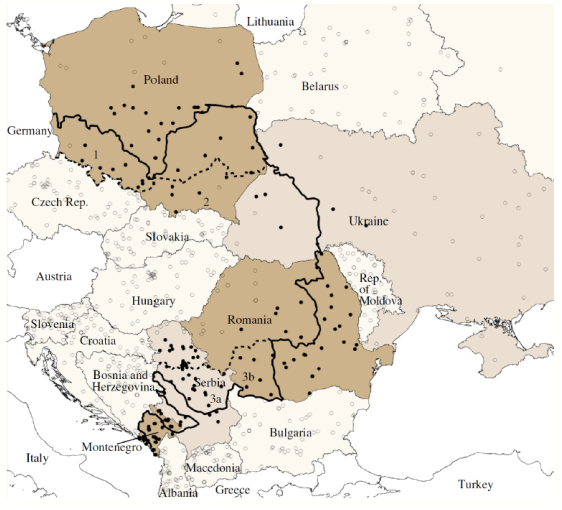
\includegraphics[width=10cm]{photos/becker.png}
    \caption{The Habsburg Empire border and the cities around it}
    \label{fig:habsburg}
\end{figure}
\begin{mdframed}

They compare how households that lived in 2006 on either side of the old Habsburg border interact with local state institutions. The Habsburg bureaucracy is described as "fairly honest, quite hard-working, and generally high-minded", the authors argue that this created trust among the citizens of the Empire in government institutions, and this trust persists over generations through continuous reciprocal behaviour.

Within a narrow range around the former border, language, culture, and geography does not change much. They exploit this set-up to uncover the effects of Habsburg institutions on trust and corruption.

They find that those who live on former Habsburg territory, have significantly higher levels of trust in courts and the policies, and are less likely to pay bribes today.

\end{mdframed}

\newpage

\begin{mdframed}
\paragraph{Acemoglu, Johnson \& Robinson (2001)} \mbox{}

    \cite{acemoglu2001} Europeans adopted very differnt colonisation policies in different colonies, with different institutions.

    In areas with high settler mortality, \textit{extractive} institutions we established to transfer resources rapidly to the metropole.

    In areas with lower settler mortality, institutions of private property we created to encourage commerce and industry.

    The authors used settler mortality as an instrumental variable (IV) for institutional quality.

    (potential) settler mortality $\Rightarrow$ settlements $\Rightarrow$ early institutions $\Rightarrow$ current institutions $\Rightarrow$ current performance

    The authors performed a two stage least squares regression, first regressing Protection Against Expropriation Risk on settler mortality, and then regressing current GDP on the predicted values from the first regression.

    They found that once you control for the effect of institutions, countries in Africa or close to the equator do not have lower incomes.
\end{mdframed}

\subsection{What did we learn?}

Other than $K$ and $H$ there may be other rivalrous production factors ($Q$) that matter for output, while the rest of output can be thought of as determined by non-rivalrous production factors.

We can distinguish between the part of $A$ that constitutes the frontier, $X$, and the efficiency at which economies operate, $E$. The frontier is linked to pure externalities and active innovation, and population growth. Efficiency is linked to how well economies allocate resources.

\newpage
\section{Intro to labour Markets}
\begin{shaded}
\subsubsection*{Notation and Facts}

\begin{itemize}
    \item [N] The total number of individuals between ages 16-64
    \item [E] Employed: Worked for one hour or more last week.
    \item [U] Unemployed: did not work AND looked for work in the last four weeks AND can start work in within the next two weeks.
    \item [I] Inactive/Nonparticipant: out of the labour force, 
    \item [L] Labour force: $L=E+U$, sum of employed and unemployed
    \[N = E + U + I = L + I\]

    \item [L/N] Participation rate: Portion of the total population (age 16-64) in the labour force.
    \item [E/N] Employment rate 
    \item [U/L] Unemployment rate
\end{itemize}

\begin{note}
    The employment rate and unemployment rate do not have the same denominator.
\end{note}
\end{shaded}

\subsection{Total Hours Per Person (THP)}

This measures the \textbf{average number of yearly hours across all individuals} and can be decomposed in to 3 terms.
\begin{enumerate}
    \item Participation Rate: $P = \frac{L}{N}$
    \item 1 minus the unemployment rate: $(1-u) = \frac{E}{L}$, the number of people in the labour force that hold a job.
    \item Hours per Worker, $h$. For someone that holds a job, the average number of yearly hours.
\end{enumerate}

\subsubsection{Unemployment}

\begin{mdframed}
    Unemployment:
    \begin{itemize}
        \item Varies across countries obviously,
        \item Varies within countries across time
        \begin{itemize}
            \item Cyclical variation: unemployment moving with business cycles (rising in recessions)
            \item Secular variation: trends in unemployment (increased in 1980s decreased in 1990s)
        \end{itemize}
        \item Persistent. Unemployment rates can remain high for decades.
    \end{itemize}
\end{mdframed}

\subsubsection{Labour of the Business Cycle}
Recall $u= \frac{U}{L} = 1-\frac{E}{L}$. This implies:
\[du = (1-u)\left[dlog\left(\dfrac{L}{N}\right) - dlog\left(\dfrac{E}{N}\right)\right]\]

Using this formula, we can decompose changes in $u$ into changes in labour force participation, and changes in employment rate.

\begin{deriv}
From $u = 1-\frac{E}{L}$ we have,
\[u = 1-\dfrac{E}{N}\dfrac{N}{L}\]
by differentiating both sides w.r.t time we obtain:
\begin{align*}
    du &= -\dfrac{E}{N}d\left(\dfrac{N}{L}\right) - \dfrac{N}{L}d\left(\dfrac{E}{N}\right) \\
        &= - \dfrac{E}{L}\dfrac{L}{N}d\left(\dfrac{N}{L}\right) - \dfrac{E}{L}\dfrac{N}{E}d\left(\dfrac{E}{N}\right) \\
        &= (1-u) \left[dlog\left(\dfrac{L}{N}\right) - dlog\left(\dfrac{E}{N}\right)\right]
\end{align*}
\begin{note}
    The last step comes from the fact that:
    \begin{align*}
        dlog\left(\dfrac{L}{N}\right) &= dlog(\left(\dfrac{N}{L}\right)^{-1}) \\
        &= -\dfrac{(\frac{N}{L})^{-2}d\frac{N}{L}}{(\frac{N}{L})^{-1}} \\
        &= -\dfrac{L}{N}d\left(\dfrac{N}{L}\right)
    \end{align*}
\end{note}
\end{deriv}

Employment and labour force participation are \textbf{procyclical} i.e decline in recessions. Employment is more procyclical than labour force participation. Additionally, rises in unemployment in recessions are driven entirely by reductions in employment.

\begin{shaded}
    DOUBLE CHECK SLIDE 16 M2-1a. THP equation $THP = h\cdot\frac{E}{N}$ or $h(1-u).$
\end{shaded}

\subsection{Neoclassical Labour Supply}

We are studying the behaviour of an individual in a market economy. The individual \textbf{sells} their labour to firms. They use their earnings to \textbf{purchase} goods from the same firm

\begin{shaded}
\subsubsection{Resources}
    The individual is endowed with $T$ units of labour e.g. 24 if measured in hours.
    \begin{itemize}
        \item If they work $h$ hours, they obtain $wh$ earnings.
        \item $w$ is the market rate of pay per unit of $h$. The worker takes this as given.
        \item The worker is allowed to work as many hours as they want.
        \item The worker also has $l=T-h$ units of leisure.
        \item They also have an amount $v$ of non-labour earnings (e.g. tax returns)
        \item Individuals can purchase goods at price $p$.
    \end{itemize}
\end{shaded}

\subsubsection{Budget Constraint}

The budget constraint can be expressed as 
\begin{equation}
\label{labour supply bc}
\begin{aligned}
    c &\leq wh + v\\
    &= wT + v - wl
\end{aligned}
\end{equation}
This arises as $h = T-l$.

\begin{figure}[h]
    \centering
    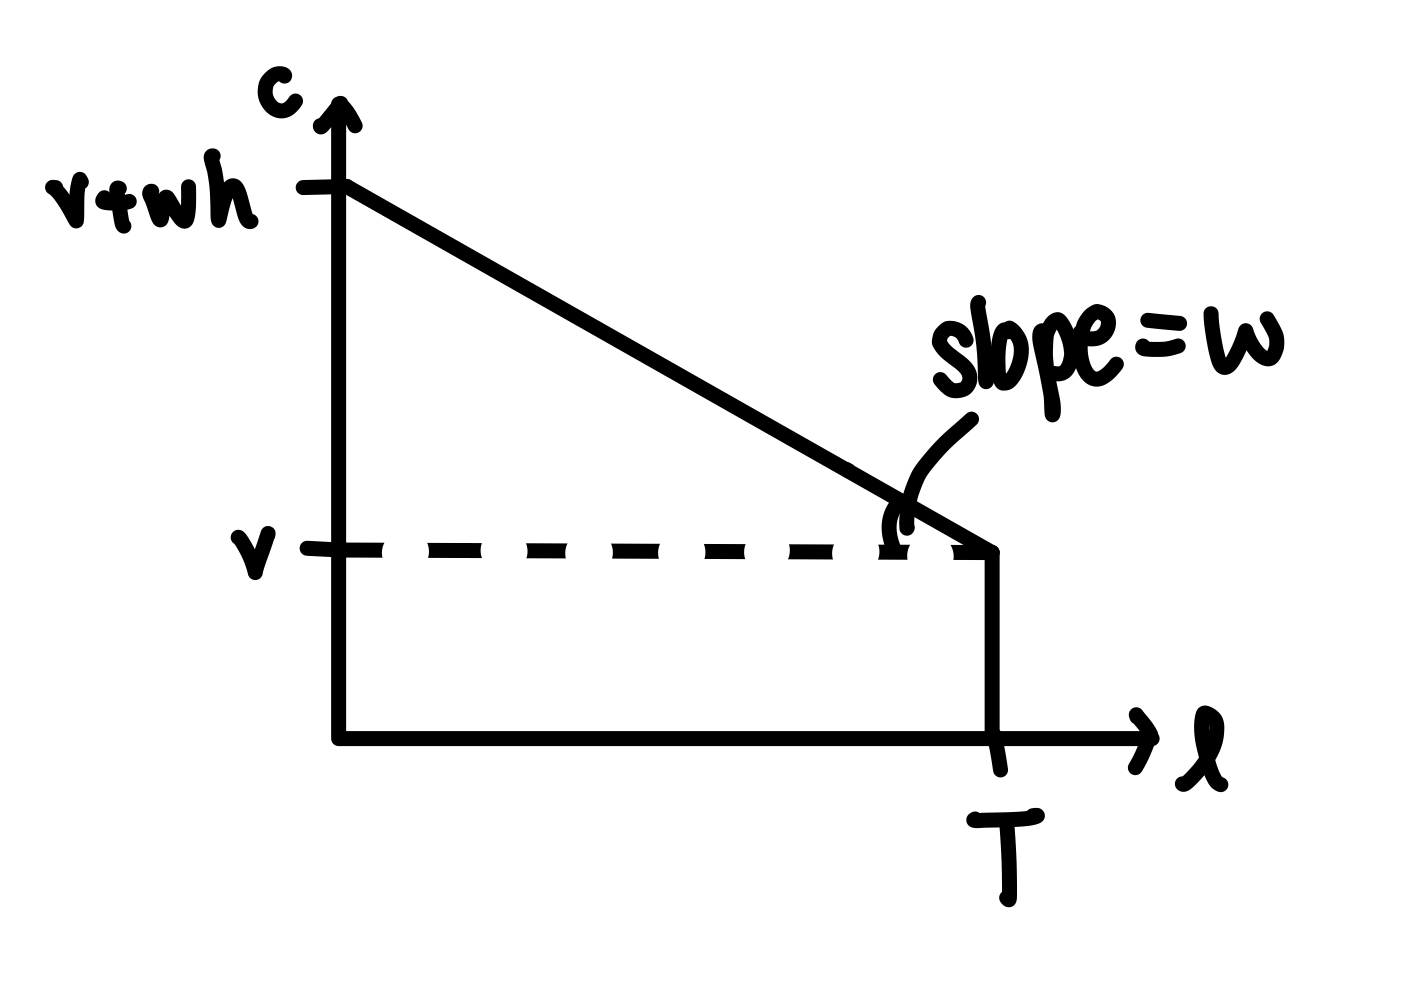
\includegraphics[width=6cm]{photos/labour bc.jpeg}
    \caption{Simple Labour Budget Constraint Diagram}
    \label{fig:labour bc}
\end{figure}

\subsubsection{Preferences}

Consuming $c$ units of output gives them $u(c,l)$ units of utility, where $u(c,l)$ satisfies the following:
\begin{itemize}
    \item More consumption and leisure improve utility: $\frac{du(c,l)}{dc}>0, \frac{du(c,l)}{dl}>0$ 
    \item Concavity
    \item Consuming nothing leads to death
    \item Working all day leads to complete exhaustion
\end{itemize}

e.g.
\begin{equation}
\label{log example}
    u(c,l) = \log (c) + \log (l)
\end{equation}

\paragraph{Indifference Curves} represent a curve, upon which any point yields the same utility and thus you are indifferent.

Given $\Bar{u}$, we implicitly define the curve $\Bar{u} = \log (c) + \log (l)$. This gives us:
\[c = e^{\Bar{u}-\log(l)} = \frac{e^{\Bar{u}}}{l}\]

\begin{figure}[h]
    \centering
    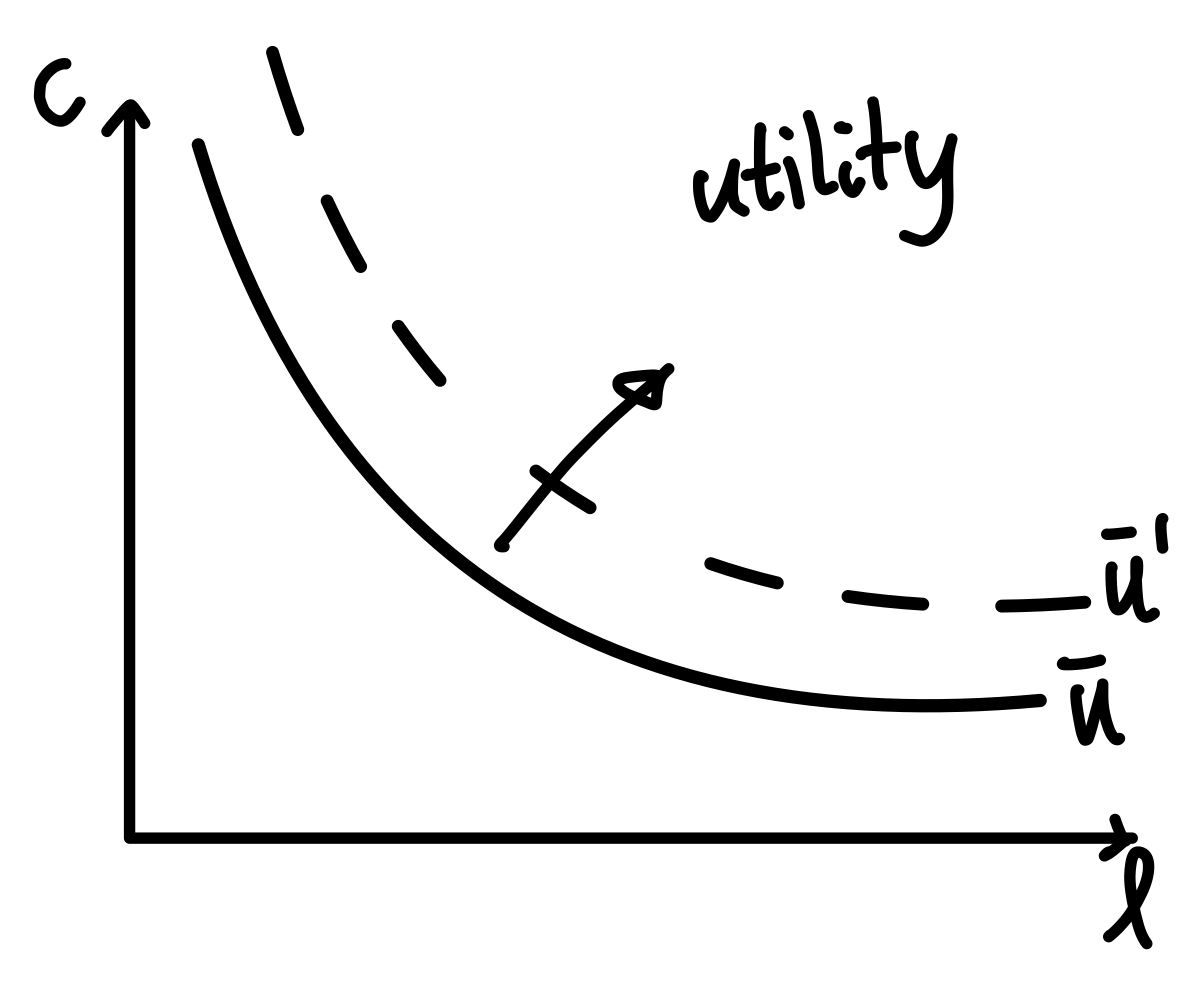
\includegraphics[width=6cm]{photos/indifference curve.jpeg}
    \caption{Indifference Curves}
    \label{fig:indifference}
\end{figure}

Any point NE of the curve is better, and given the opportunity will always move to that point. Therefore, we maximise utility when our indifference curve is tangent to the budget constraint. In Figure \ref{fig:indifference} $\Bar{u}^\prime$ is better than $\Bar{u}$.

\begin{note}
    The slope of this curve equals: $-\dfrac{\frac{du(c,l)}{dl}}{\frac{du(c,l)}{dc}}$. This is the marginal rate of substitution (MRS).
\end{note}
\begin{deriv}
\[u(c,l) = \Bar{u}\]
differentiating both sides w.r.t $l$,
\begin{gather*}
    \dfrac{du(c,l)}{dc}\dfrac{dc}{dl} + \dfrac{du(c,l)}{dl} = 0 \\
    \dfrac{dc}{dl} = -\dfrac{\frac{du(c,l)}{dl}}{\frac{du(c,l)}{dc}}
\end{gather*}
\end{deriv}

\subsubsection{Consumer Problem}

Given their possibilities they want to obtain as much utility as possible. This is equivalent to the following constrained maximisation problem:
\[\underset{c,l}{max} \  u(c,l) \text{ s.t. } c\leq wT + v - wl\]
with $l\in [0,T], c\geq0$.

\subsubsection{Solutions}
\paragraph{Graphical Solution} \mbox{} \\

\begin{figure}[h]
    \centering
    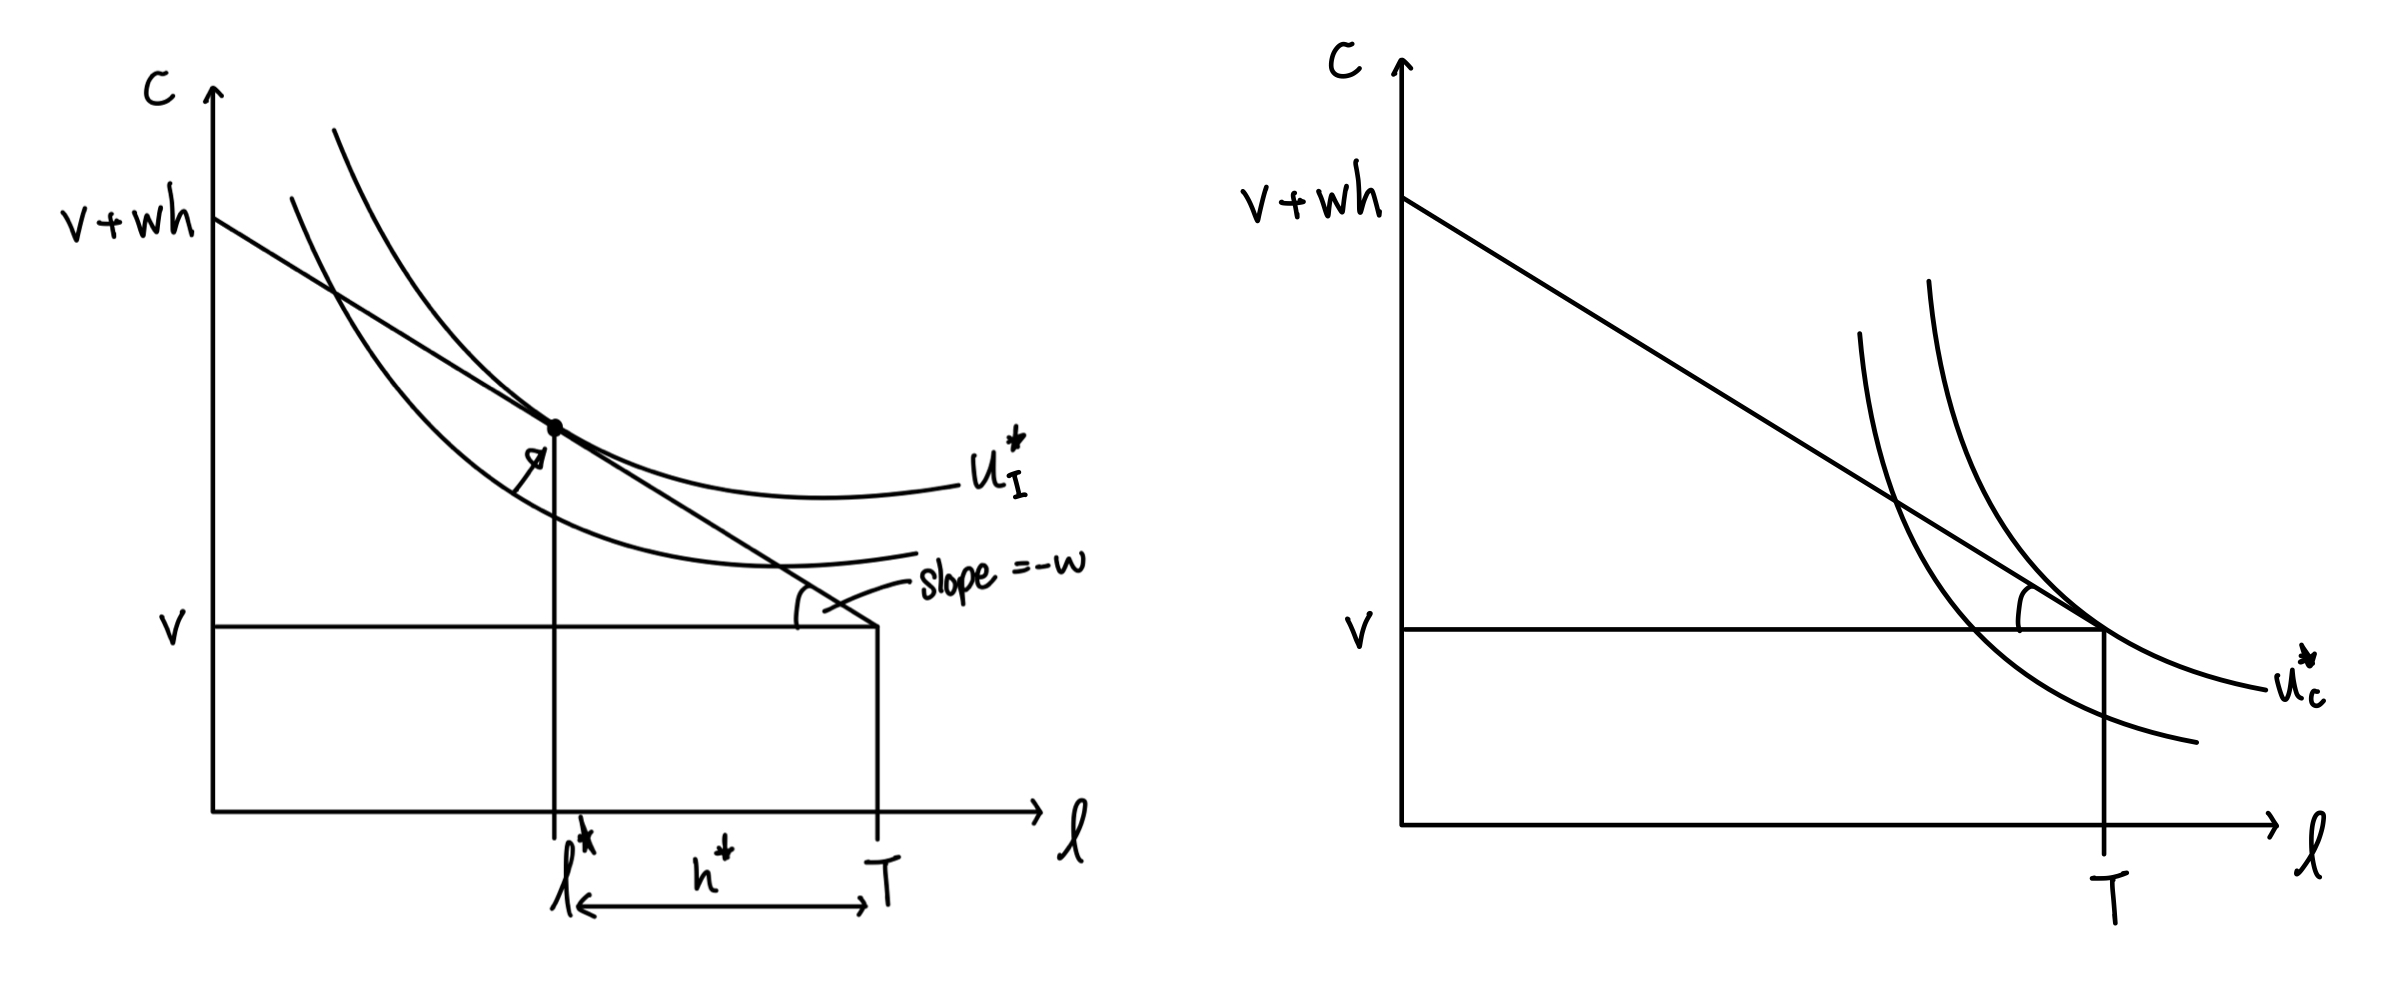
\includegraphics[width=15cm]{photos/interior-corner solution.jpeg}
    \caption{Graphical Solutions: Interior and Corner}
    \label{fig:interior corner sol}
\end{figure}

As you can see from figure \ref{fig:interior corner sol} we can have both interior and corner solutions. The graphs are only representations of the solutions, we are unable to find solutions from the graph but rather use them to present the solutions found in the following methods.

We have an interior solution when $h^*>0$ and a corner solution when $h^*=0$

\paragraph{Substitution method} \mbox{} \\

For optimal solutions we cannot have any waste, and therefore the budget constraint is $c=xT+v-wl$ rather than the looser $\leq$. We can substitute this in to the utility function, giving us the maximisation problem:
\[\underset{l}{max}\ u(wT + v - wl, l)\]

This is a concave function so an interior solution can be found by differentiating w.r.t $l$. 
\begin{note}
    If this method leads to an inconsistent solution, then we have a corner solution.
\end{note}

The first order condition (FOC) for this problem is:
\[-\dfrac{du(wT+v-wl, l)}{dc}w + \dfrac{du(wT+v-wl,l)}{dl} = 0\]

In the example of the log case \eqref{log example}:
\begin{gather*}
    \dfrac{w}{wT+v-wl}-\dfrac{1}{l} = 0 \\
    \dfrac{w}{wT+v-wl} = \dfrac{1}{l} \\
    wl = wT+v-wl \\
    2wl = wT+v \\
    l^* = \dfrac{wt+v}{2w} \\
    \text{substituting back in } c^* = \dfrac{wT + v}{2}
\end{gather*}

This solution is valid if $\frac{wt+v}{2w}\leq T$, if not then we have a corner solution, $l^* = T, c = v.$

\subsection{Simple Income and Substitution Effects}

We want to assess what happens when $w$ increases. A wage increase is like decreasing the price of goods w.r.t leisure. i.e. leisure becomes more expensive because the wage is increased and therefore the opportunity cost of leisure is higher.

For simplicity, we will assume $v=0$.

\newpage

\begin{figure}[h]
    \centering
    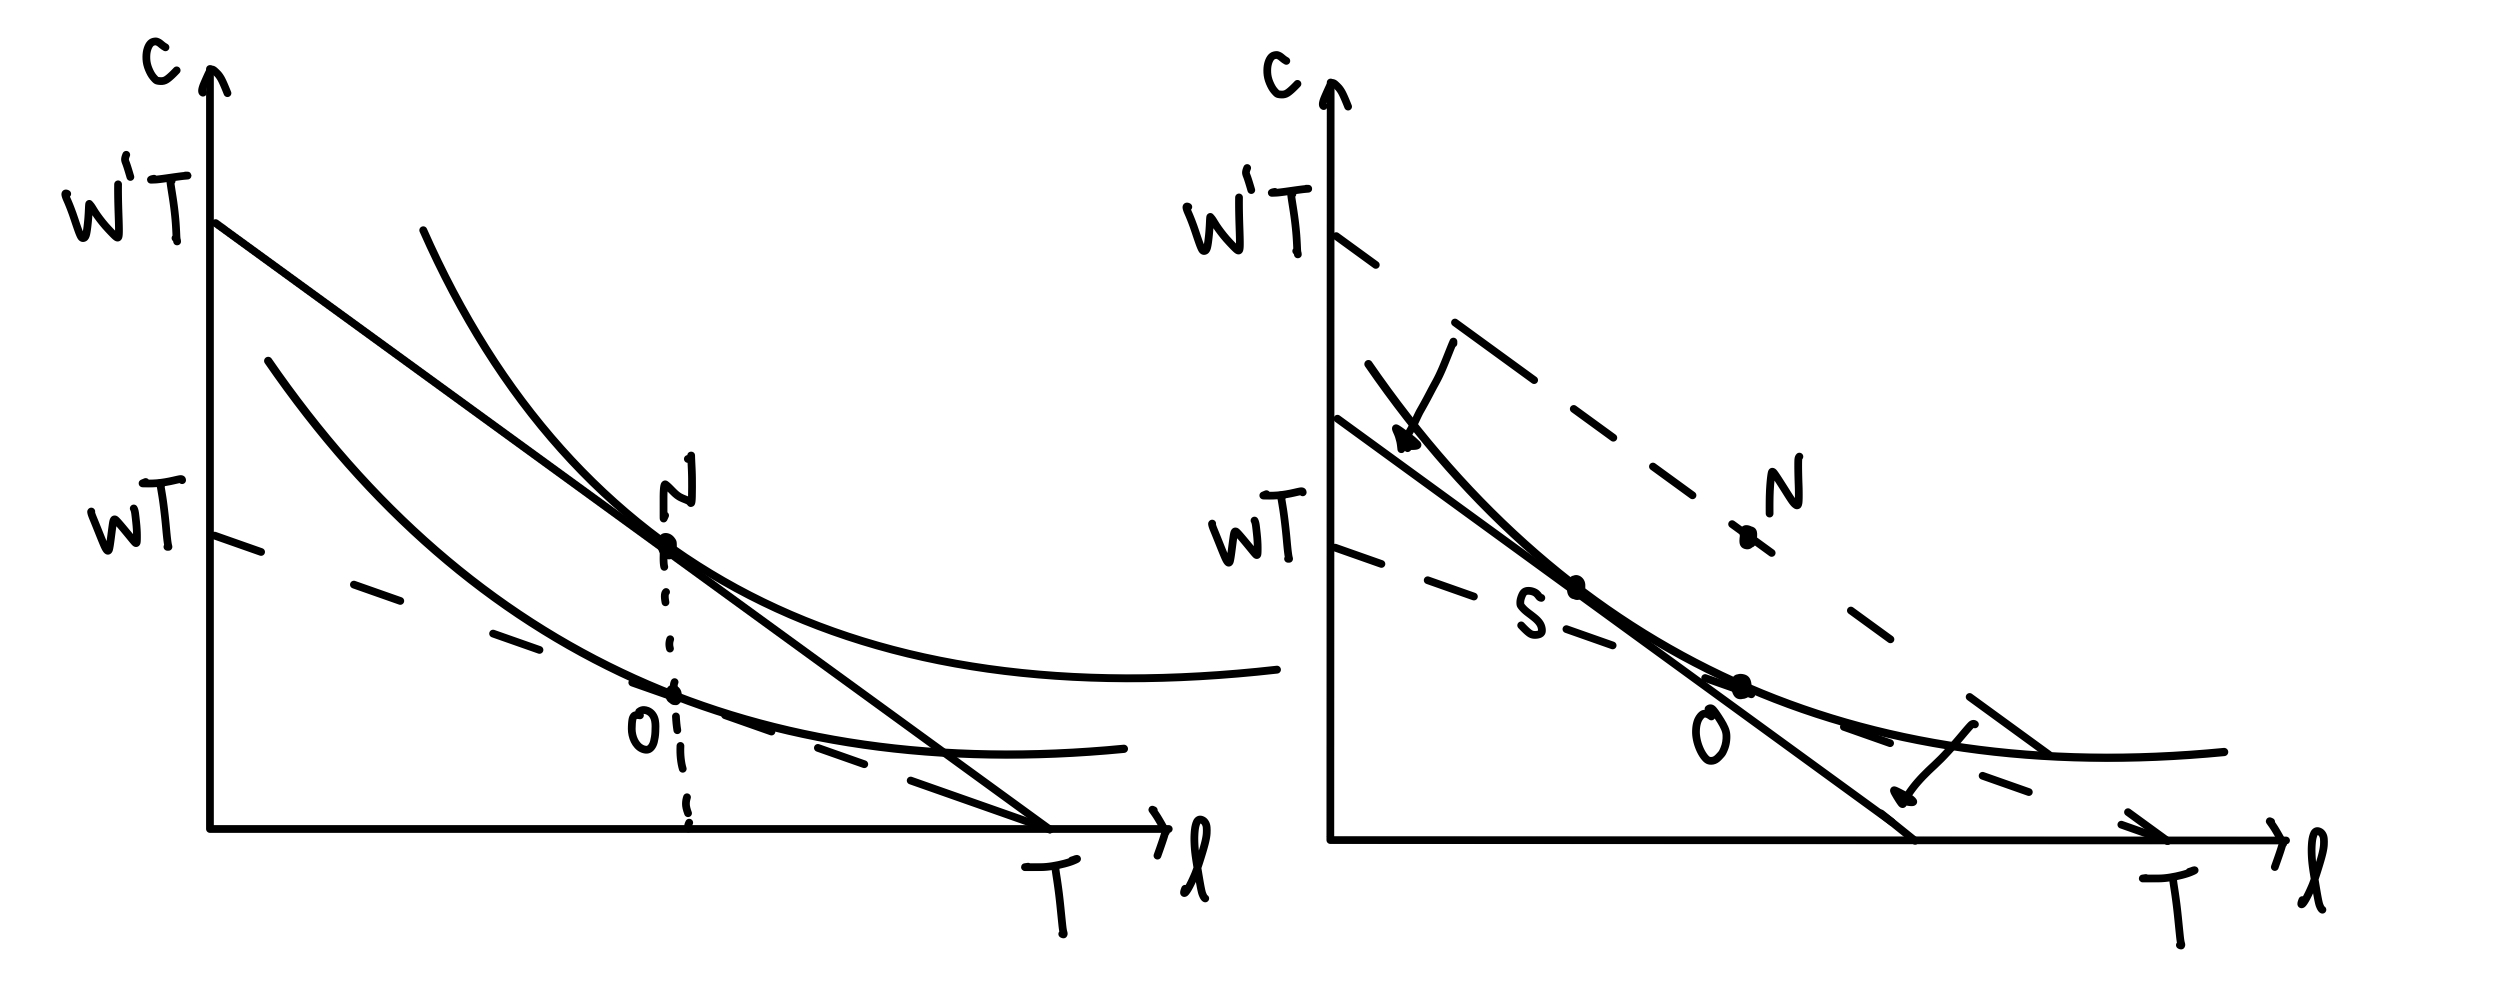
\includegraphics[width=12cm]{photos/inc sub effect.jpeg}
    \caption{Full Effect broken down in to Substitution and Income Effects}
    \label{fig:sub inc effect}
\end{figure}

What we see in the LHS of Figure \ref{fig:sub inc effect} is the full effect of an increase in $w$. We see that an increase in $w$ leads to an increase in $c$ and the equilibrium point shifts from $O$ to $N$. 
We can break down this full effect in to income and substitution effects.

\begin{mdframed}
    The substitution effect focuses on the change in price. This is done through keeping utility constant, but implement the new budget constraint. So we shift the new budget constraint downward until it is tangent with the original indifference curve. We see a decrease in leisure and an increase in consumption, and an equilibrium point moving from $O$ to $S$.
    \begin{intu}
        The cost of leisure has increased due to the increase in wages. Because of this intuitively they decrease leisure.
    \end{intu}

    The income effect focuses on the change in purchasing power. To measure the income effect, we compare the fictitious budget constraint line use in the substitution effect with the real new budget constraint, both with slope $-w^\prime$. Moving from $S$ to $N$ is the income effect. We see that we have both more leisure and more income.
\end{mdframed}

\begin{note}
    In our case, the full effect is directly above the original equilibrium because we have specified our model in the \textbf{log utility case}, with $v=0$. In this specific case, the income and substitution effects exactly cancel out.
\end{note}

Is this reasonable? We've seen that economies are getting richer and richer ($\uparrow w$) and we have seen in countries like the US hours worked have stayed fairly consistent over this time. However, what we have seen in the UK and mainland Europe, have actually seen a decrease in hours worked. This implies that the income effect dominates in these countries.

\newpage
\section{Labour Supply}

As we saw in the Intro to Labour Markets section, labour supply is determined by the income and substitution effects. We will look at these effects in more detail now.

\subsection{Income and Substitution Effects}

\subsubsection{Increase in non-labour income}
Before we were discussing when $v=0$, now we will talk about when $v>0$. If there is an increase in $v$ we will see only income effects and no substitution effects.
\begin{intu}
    Because wage is not changing, there is no change to the opportunity cost of leisure.
\end{intu}

\begin{figure}[h]
    \centering
    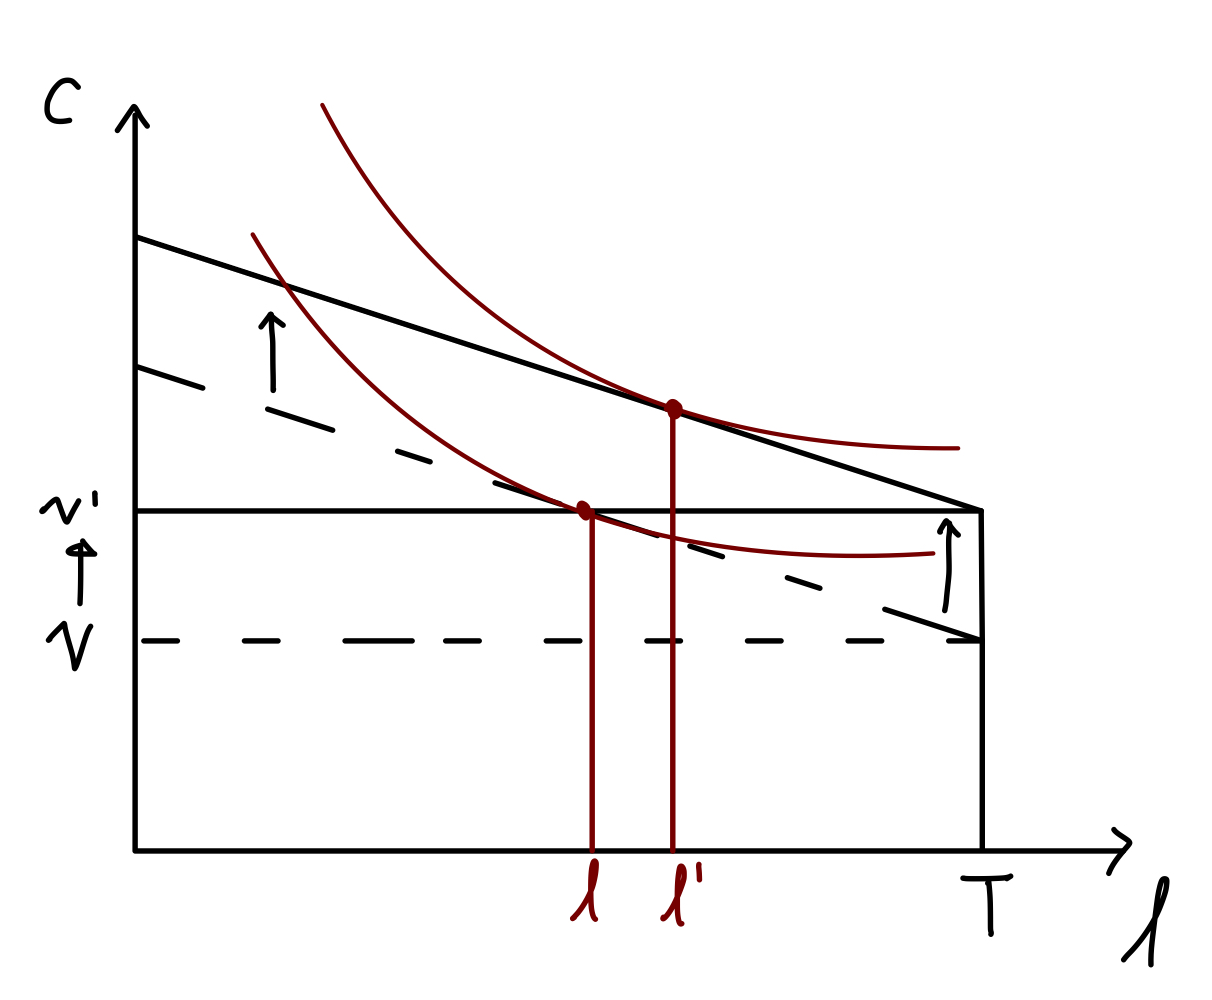
\includegraphics[width=10cm]{photos/shift in v.jpeg}
    \caption{Increase in non-labour income, v}
    \label{increase in v}
\end{figure}
This income effect means that the individual will increase their leisure and therefore work less.

\begin{example}
With log-utility we have:
\[\dfrac{\partial l^*}{\partial v} = \dfrac{1}{2w}>0\]
\end{example}

\subsubsection{Increase in Wage}
In this case, there are both income and substitution effects. 
\begin{intu}
    This is because now with the increase in wages, we have an increase in the cost of leisure. We must find how individuals substitute their consumption-leisure balance.
\end{intu}

\begin{figure}[h]
    \centering
    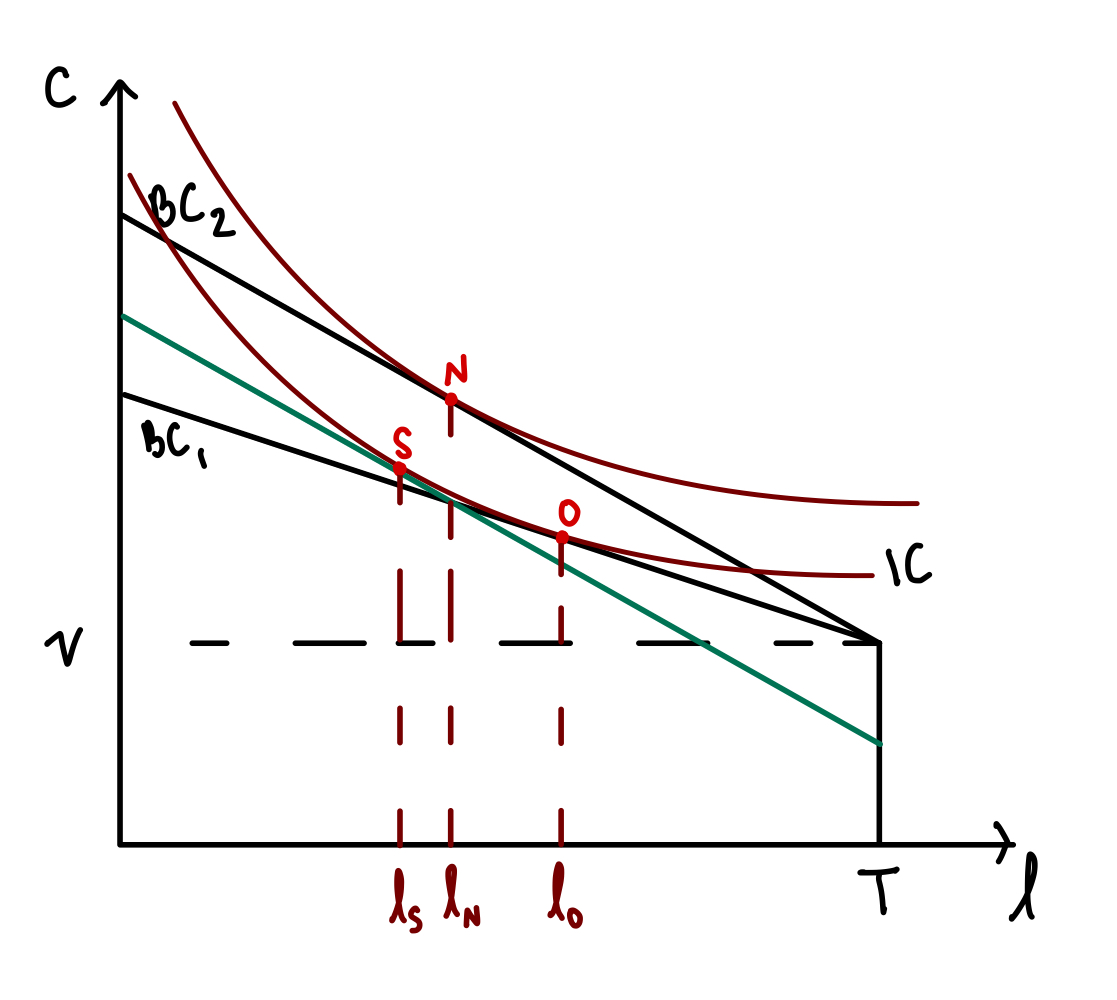
\includegraphics[width=10cm]{photos/shift in w.jpeg}
    \caption{Increase in Wage}
    \label{fig:increase in w}
\end{figure}

An increase in wage manifests itself as an increase in the slope of the budget constraint. We can identify both the income effects and the substitution effects within this change through some interesting tricks.

\begin{deriv}
    From point $O$ to point $N$ we have the original and new levels of consumption and leisure. 
    
    If we were to shift the new budget constraint line denoted $BC_2$ down tangentially to the old utility curve this would give us the \textcolor{OliveGreen}{green line}. This line is a hypothetical budget constraint.
    \begin{intu}
        Given my \textbf{new} wage and \textbf{old} utility, how would my leisure and consumption change?
    \end{intu}

    Our substitution effect is the change from $l_O \rightarrow l_S$.

    The income effect is simply the change from our fake budget constraint at point $S$ and our new point $N$. The income effect is the change from $l_S \rightarrow l_N$
\end{deriv}

\begin{example}
To see which effect dominates we find the derivative of $l^*$ w.r.t $w$. With our example log-utility function, the substitution effect will dominate:
    \[\dfrac{\partial l^*}{\partial w} = \dfrac{T}{2w} - 2\dfrac{wT+v}{(2w)^2}= -2\dfrac{v}{4w^2}<0\]
    because both $v,w$ are both positive.
\end{example}

We have an exception though. When we had a corner solution prior to the wage increase, there is only substitution effects at play $\dfrac{\partial l^*}{\partial w}\leq0$.

\begin{figure}[h]
    \centering
    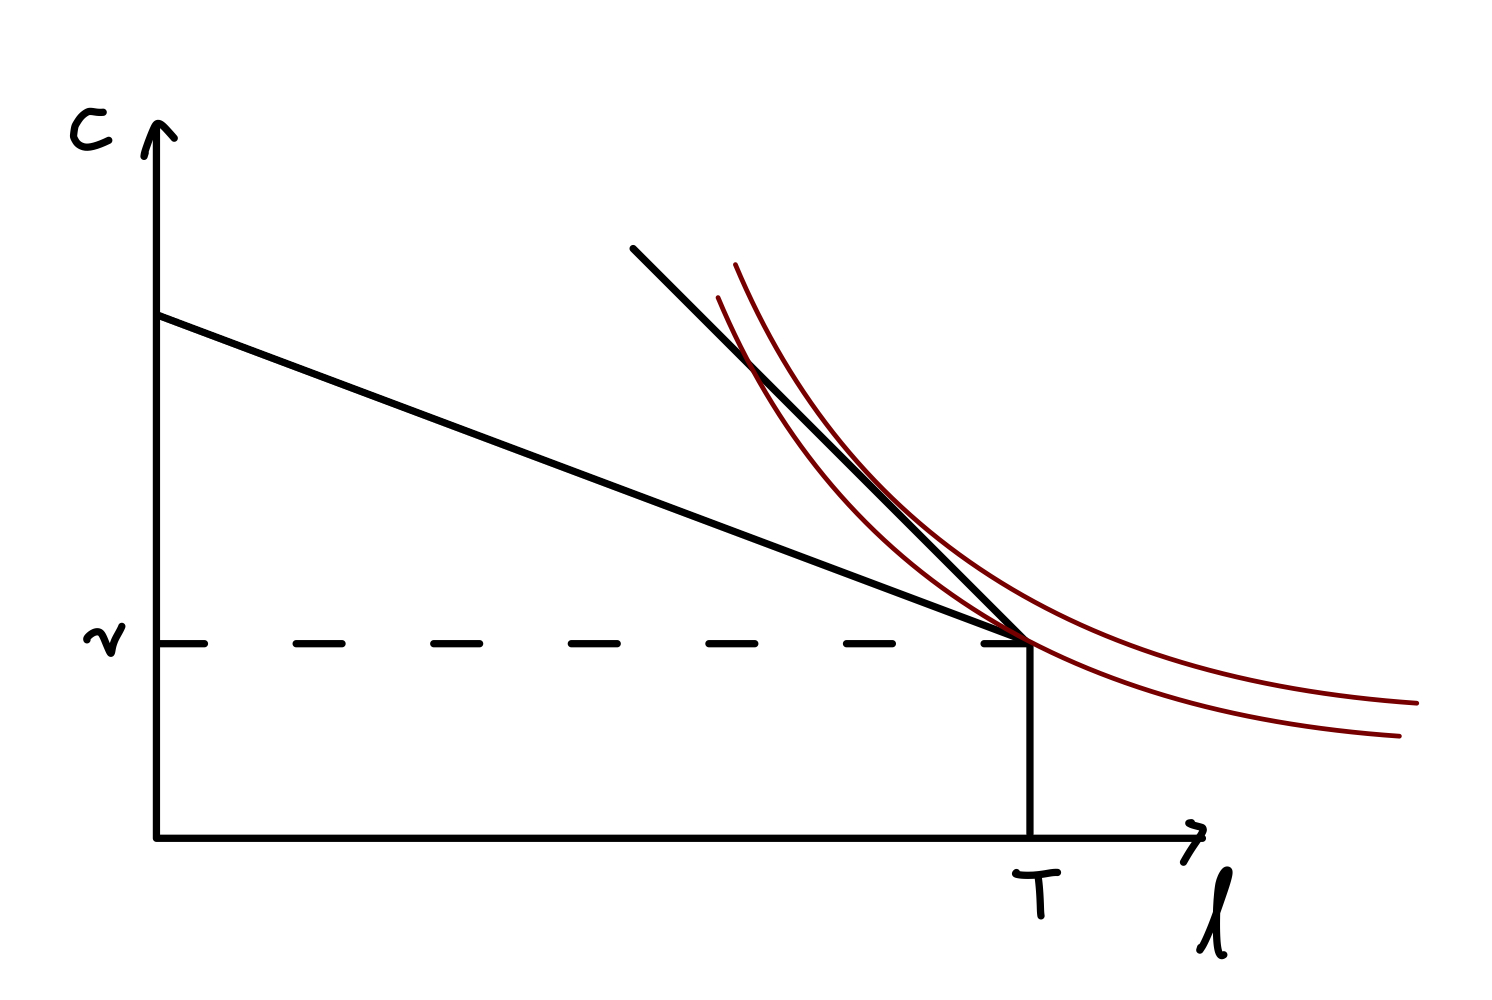
\includegraphics[width=10cm]{photos/corner solution.jpeg}
    \caption{Exception: Corner Solution}
    \label{corner solution}
\end{figure}

You can see that an individual who had a corner solution would strictly be better by decreasing their leisure as the new budget constraint crosses the original utility curve twice. By shifting the utility curve and seeing the intersection with the new budget constraint you can see that they will enter the labour force.

If we increase the wage $w$, eventually the individual decides to work. 
\begin{definition}
\textbf{Reservation wage}: the minimum wage that induces the individual to work.

We can find $w^R$ using:
\begin{align*}
    \dfrac{w^R T + v}{2w^R} &= T \\
    w^R &= \dfrac{v}{T}
\end{align*}
\end{definition}

\subsubsection{Proportional Increases}
If $\uparrow v$ and $\uparrow w$ by the same proportion ($w^\prime = \rho w, v^\prime = \rho v$), there are both income and substitution effects, so the overall change in $l$ is ambiguous.

\begin{example}
    With log utility the two proportional increases will exactly cancel out:
    \[l^* = \dfrac{\rho wT + \rho v}{2 \rho w} = \dfrac{wT+v}{2w}\]
\end{example}

\subsubsection{Labour Supply Curves}
\begin{mdframed}
    Watch Lecture to see what he does in this section.
\end{mdframed}

The labour supply curve is increasing (decreasing) if the substitution (income) effect dominates.

\begin{example}
    In most developed countries, income effects seem to dominate in the long run.
\end{example}

\subsubsection{Economic Growth and Labour Supply}

In the process of developing many countries experienced large increases in hours initially. This leads to the \textit{backward bending} labour supply curve below. When wage is low the substitution effect dominates, and when wage is high the income effect dominates.

\begin{figure}[h]
    \centering
    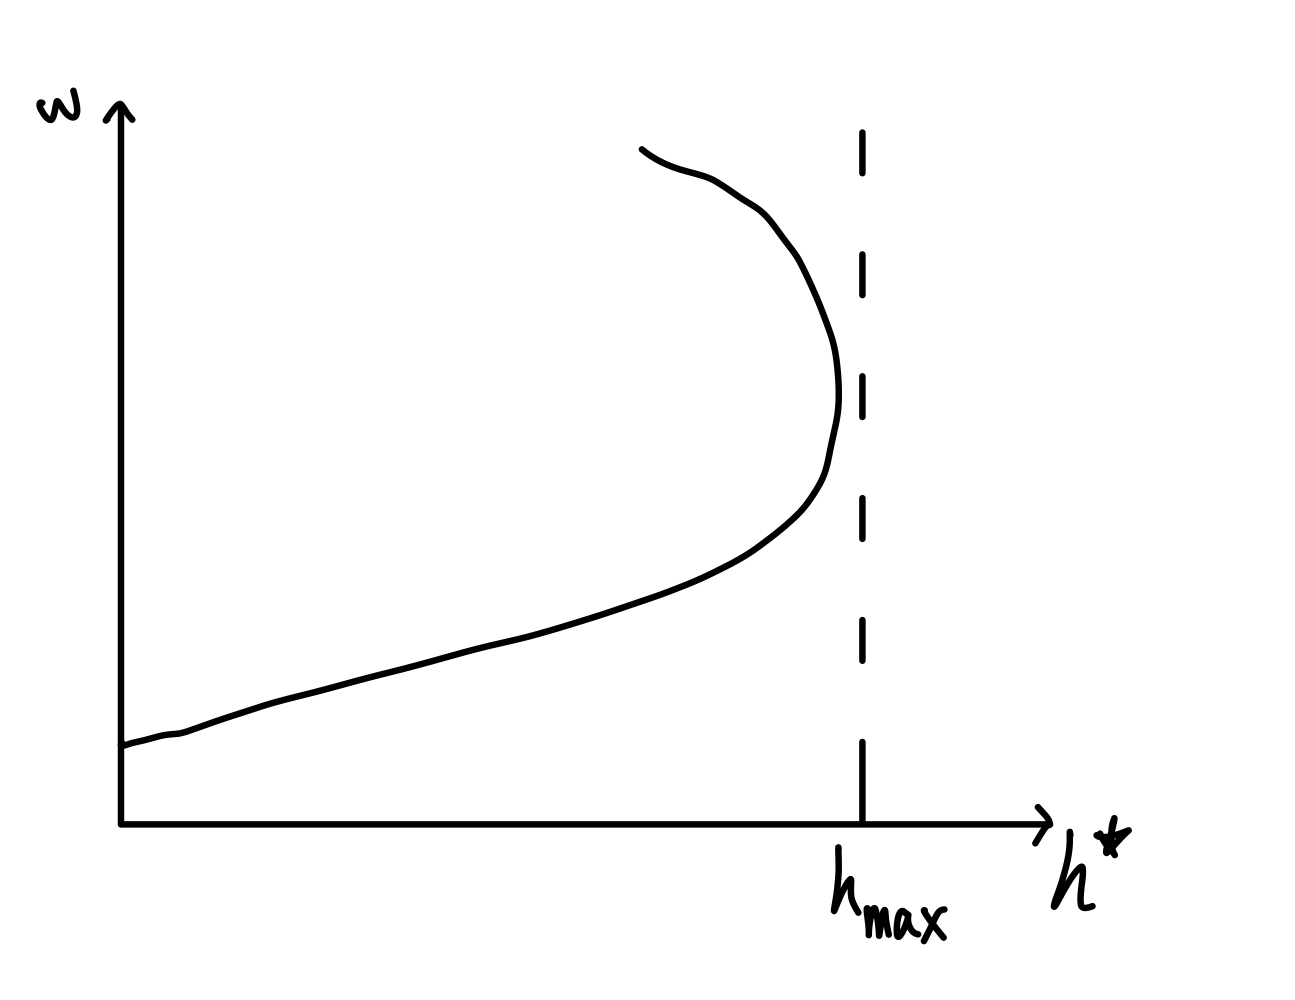
\includegraphics[width=10cm]{photos/backward bending labour supply.jpeg}
    \caption{Backward Bending Labour Supply Curve}
    \label{fig:backward bending labour supply curve}
\end{figure}

\subsection{Over the Business Cycle}

We saw that in the long-run the income effect seems to dominate in developed countries, implying:
\[\dfrac{\partial h}{\partial w}\leq0\]

Now we must assess this relationship in the short run, at business cycle frequencies. In the data, we tend to see that total hours worked moves in a very similar fashion to GDP, while real wages fluctuate much more than GDP.

\begin{figure}[h]
    \centering
    \subfloat[\centering Deviations in Total Hours Worked and GDP from their Trends]{{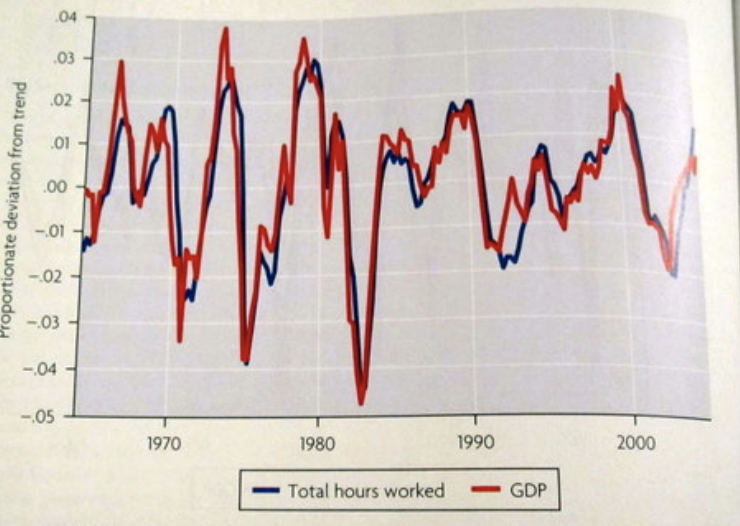
\includegraphics[width=7cm]{photos/hours worked and GDP.png} }}%
    \qquad
    \subfloat[\centering Deviations in Real Wages and GDP from their Trends]{{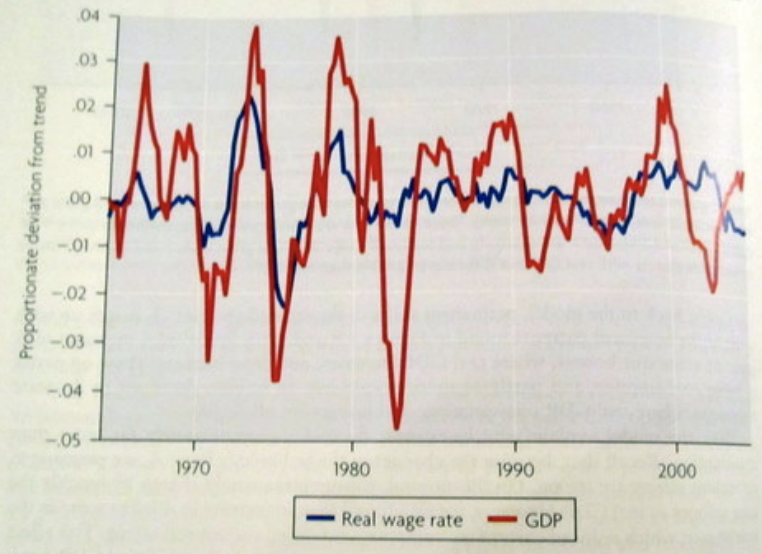
\includegraphics[width=7cm]{photos/wage and GDP.png} }}%
    \caption{Total Hours Worked and Real Wage fluctuations relative to GDP}%
    \label{fig:panel format}%
\end{figure}
\begin{intu}
    In booms, GDP $\uparrow$, THP $ \uparrow$ and $w\uparrow$. This makes THP and $w$ \textbf{procyclical}. 
    
    This suggests that at business cycle frequency substitution effects dominate: in booms wages increase and total hours worked increase.
\end{intu}

\newpage

\subsubsection{2-Period Model}

For simplicity, individuals do not have \textit{non-labour income} ($v_1 = 0, v_2=0$). Working each period entails a \textit{rate of pay} $w_1, w_2$ respectively. Finally, individuals have access to \textit{savings}. Saving $s_1$ units today yields $s_1$ to use tomorrow. We assume that the interest rate is 0.

Our budget constraints for this problem can be described as:
\begin{equation}
\begin{aligned}
c_1+s_1 & =w_1\left(T-l_1\right) \\
c_2 & =w_2\left(T-l_2\right)+s_1
\end{aligned}
\end{equation}
\begin{note}
    There is no savings decision in period 2 ($s_2 = 0$).
\end{note}

Individuals have preferences over consumption and leisure in both periods, $c_1, c_2, l_1, l_2$:
\begin{equation}
U\left(c_1, c_2, l_1, l_2\right)=u\left(c_1\right)+\rho\left(l_1\right)+u\left(c_2\right)+\rho\left(l_2\right)
\end{equation}
where $u(.)$ and $\rho(.)$ are \textit{increasing and concave} and have infinite marginal utility at zero.
\begin{note}
    We assume no discounting. People value future consumption the same they do today, and preferences are separable.
\end{note}

This individual's problem can be described as:

\begin{equation}
\begin{array}{rl}
\underset{c_1, c_2, l_1, l_2, s_1}{\max} & U\left(c_1, c_2, l_1, l_2\right) \\
\text { s.t. } & \\
c_1+s_1 & \leq w_1\left(T-l_1\right) \\
c_2 & \leq w_2\left(T-l_2\right)+s_1
\end{array}
\end{equation}
Because we know that in equilibrium the budget constraints will be satisfied at equality, we can combine them into a single equation.
\begin{equation}
    \label{lifetime budget constraint}
    c_1 + c_2 = w_1(T-l_1) + w_2(T-l_2)
\end{equation}
This is called the lifetime budget constraint. We can now solve this problem as a Lagrangian.

\begin{equation}
\begin{aligned}
\max _{c_1, c_2, l_1, l_2, \lambda} L & =u\left(c_1\right)+\rho\left(I_1\right)+u\left(c_2\right)+\rho\left(I_2\right) \\
& +\lambda\left[w\left(T-l_1\right)+w_2\left(T-l_2\right)-c_1-c_2\right]
\end{aligned}
\end{equation}

We get the following results:
\begin{align*}
    \dfrac{\partial L}{\partial c_1}&: u^\prime (c_1) = \lambda \\
    \dfrac{\partial L}{\partial c_2}&: u^\prime (c_2) = \lambda \\
    \dfrac{\partial L}{\partial l_1}&: \rho^\prime (l_1) = \lambda w_1 \\
    \dfrac{\partial L}{\partial l_2}&: \rho^\prime (l_2) = \lambda w_2
\end{align*}

    \paragraph{Consumption Smoothing}: \mbox{}
    \[u^\prime (c_1) = u^\prime (c_2)\]
    which implies $c_1 = c_2$.
    \begin{note}
        This is independent of wage ($w_1,w_2$). The individual uses borrowing/savings to achieve this.
    \end{note}
    This is because of concavity.

\begin{figure}[h]
        \centering
        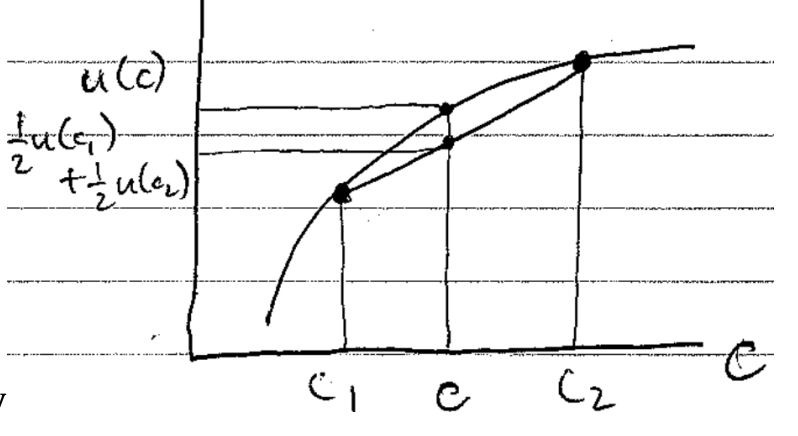
\includegraphics[width=8cm]{photos/consumption smoothing.png}
        \caption{Caption}
        \label{fig:my_label}
\end{figure}

    \paragraph{Permanent Income Hypothesis:} \mbox{}

    \begin{equation}
2 c=c_1+c_2=w_1\left(T-l_1\right)+w_2\left(T-l_2\right)
\end{equation}
Consumption depends on "permanent income" rather than current income. 

\begin{definition}
    \textbf{Permanent Income:} the discounted sum of the income in all periods.
\end{definition}


\paragraph{Labour Choices:} \mbox{}

    \begin{equation}
\begin{aligned}
& \rho^{\prime}\left(I_1\right)=u^{\prime}(c) w_1 \\
& \rho^{\prime}\left(I_2\right)=u^{\prime}(c) w_2 \\
\Rightarrow& \rho^{\prime}\left(I_1\right)=\frac{w_1}{w_2} \rho^{\prime}\left(I_2\right)
\end{aligned}
\end{equation}

If we apply this to our business cycle example: let us assume period 1 is a boom and period 2 is a recession ($w_1>w_2 \Rightarrow \frac{w_1}{w_2}>1$).

Now that we have this assumption, we can substitute this to our previous equation which gives us:
\[\rho^\prime(l_1) > \rho^\prime(l_2)\]

Because we know that $\rho^\prime(.)$ is concave, meaning it is decreasing in leisure, $\rho^\prime(l_1) > \rho^\prime(l_2)$ implies $l_1 <l_2$.

This implies that labour supply is pro-cyclical ($h_1>h_2$) and \textbf{substitution effects dominate}.


\begin{intu}
    Income effects depend on "permanent income" and thus are "small":
    \begin{equation}
c=\frac{w_1\left(T-l_1\right)+w_2\left(T-l_2\right)}{2}
\end{equation}

Substitution effects depend only on current wages and thus are "strong"
\begin{equation}
\frac{u^{\prime}\left(c_1\right)}{\rho^{\prime}\left(l_1\right)}=\frac{1}{w_1}
\end{equation}
\end{intu}

\subsection{Long-Run Model}
\subsubsection{Setup}

\begin{deriv}
Let us assume log utility:
\begin{equation}
U\left(c_1, c_2, I_1, l_2\right)=\log \left(c_1\right)+\log \left(I_1\right)+\log \left(c_2\right)+\log \left(I_2\right)
\end{equation}
which leads to the following conditions
\begin{equation}
\begin{aligned}
c & =\frac{w_1\left(T-l_1\right)+w_2\left(T-l_2\right)}{2} \\
c_1 & =c=w_1 l_1 \\
c_2 & =c=w_2 l_2
\end{aligned}
\end{equation}
Substituting $c_1,c_2$ in to our equation for $c$, we get:
\begin{equation}
\begin{aligned}
c & =\frac{w_1\left(T-\frac{c}{w_1}\right)+w_2\left(T-\frac{c}{w_2}\right)}{2} \\
& =\frac{w_1 T+w_2 T}{2}-\frac{c+c}{2}.
\end{aligned}
\end{equation}

We can now solve for $c,l_1,l_2$.
\begin{equation}
\begin{aligned}
& c=\frac{w_1 T+w_2 T}{4} \\
& l_1=\frac{w_1 T+w_2 T}{w_1 4} \\
& l_2=\frac{w_1 T+w_2 T}{w_2 4}
\end{aligned}
\end{equation}
\end{deriv}

\subsubsection{Many Years Apart}

We will compare an economy many years apart:
\begin{itemize}
    \item Person 1 (grandfather) $w_1$ and $w_2$
    \item Person 2 (grandson) $w_1^\prime = (1+g)w_1, w_2^\prime = (1+g)w_2$
    \item Person 2 was born many years later than Person 1, and consequently has higher wages due to economic growth.
\end{itemize}

It follows that:
\begin{equation}
\begin{aligned}
l_1^{\prime} & =\frac{w_1^{\prime} T+w_2^{\prime} T}{w_1^{\prime} 4}=\frac{w_1(1+g) T+w_2(1+g) T}{w_1(1+g)^4} \\
& =\frac{w_1 T+w_2 T}{w_1 4}=l_1
\end{aligned}
\end{equation}

Therefore, with log-utility economic growth $(1+g)$ has no effect on work choices, just like the static model. With more general preferences, income or substitution effects could dominate.

\subsection{Labour Market Equilibrium}

\subsubsection{Supply}
We can express the short-run labour supply using the following graph

\begin{figure}[h]
    \centering
    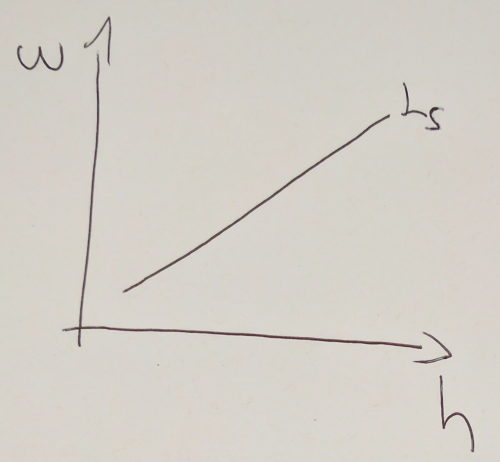
\includegraphics[width=10cm]{photos/short run labour supply.png}
    \caption{Short Run Labour Supply}
    \label{fig:short run labour supply}
\end{figure}

\subsubsection{Demand}
We must find the labour market demand to close the labour market equilibrium. We look at the problem of the neoclassical firm to determine the labour demand.

\[\underset{L}{\max}AF(L,K) - wL\]

\begin{note}
    We assume in the "short-run" the capital stock is fixed, so firms can only choose $L$.
\end{note}

We can safely assume that output is an increasing function of labour, which exhibits decreasing marginal returns to labour. That is:
\begin{equation}
\frac{d F(L, K)}{d L}>0 \text { and  } \frac{d^2 F(L, K)}{(d L)^2}<0
\end{equation}

The solution to this problem is a downward-sloping labour demand curve:
\begin{equation}
A \frac{d F(L, K)}{d L}=w
\end{equation}

\begin{figure}[h]
    \centering
    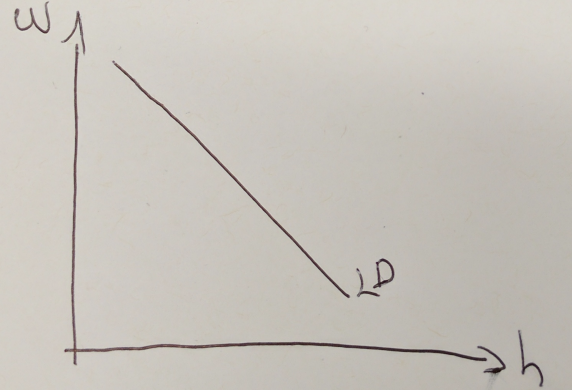
\includegraphics[width=10cm]{photos/short run labour demand.png}
    \caption{Short Run Labour Demand}
    \label{fig:short run labour demand.}
\end{figure}

\begin{example}
    \begin{equation}
\text { if } F(L, K)=L^\alpha K^{1-\alpha} \text { then } L=K\left[\frac{A \alpha}{w}\right]^{\frac{1}{1-\alpha}}
\end{equation}
\end{example}
\subsubsection{Equilibrium}
Obviously where the curves in Figures \ref{fig:short run labour supply} \ref{fig:short run labour demand.} cross will be the short-run labour market equilibrium.

\begin{figure}[h]
    \centering
    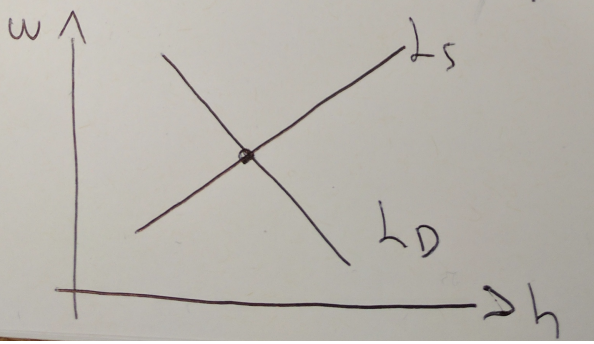
\includegraphics[width=10cm]{photos/short run labour market equilibrium.png}
    \caption{Short run Labour Market Equilibrium}
    \label{fig:labour market equilibrium}
\end{figure}

To explain the behaviour of labour over the business cycle we appeal to the \textbf{"Real business cycle theory"}. This states shocks to $A$ drive the business cycle, e.g. internet revolution in the 90s.

An increase in $A$ will lead to an increase in labour demand, but obviously no shift in labour supply.

\begin{figure}[h]
    \centering
    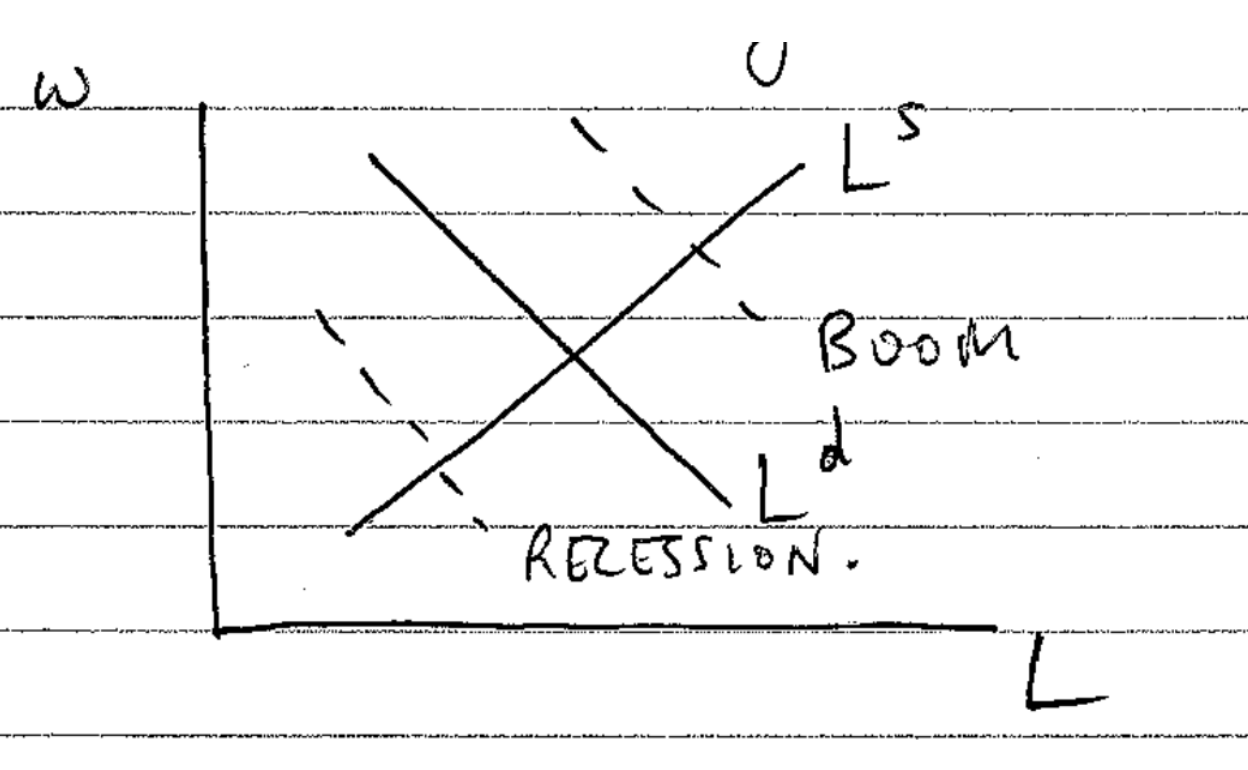
\includegraphics[width=10cm]{photos/labour market shocks to A.png}
    \caption{Shocks to technology leading to increases/decreases in labour demand}
    \label{fig:labour market shocks}
\end{figure}


\newpage

\section{Efficiency Wages (NSC)}

\subsubsection{Employment over the Business Cycle}

\begin{figure}[h]
    \centering
    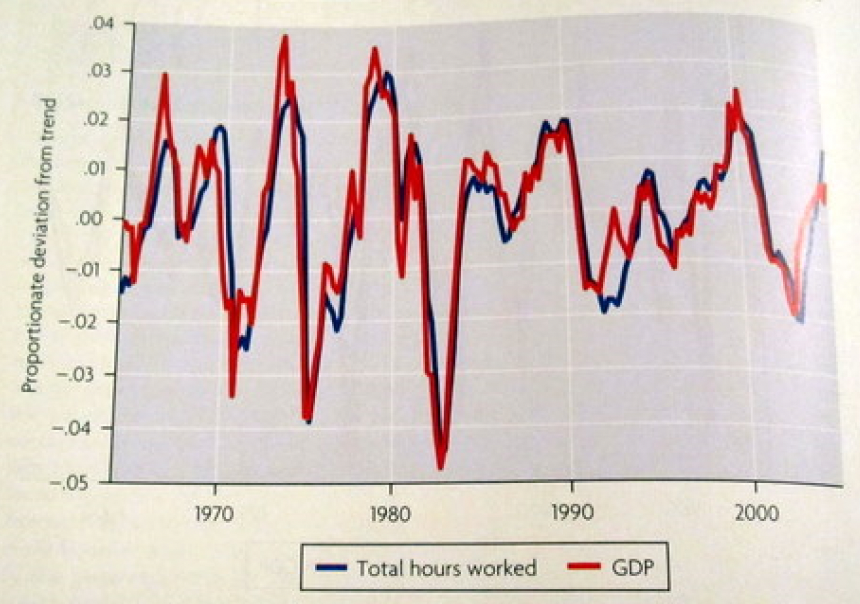
\includegraphics[width=10cm]{photos/labour force vs gdp.png}
    \caption{Deviations from GDP and Labour force from their respective trends}
    \label{fig:labour force vs gdp}
\end{figure}

From our neoclassical model $A_t \uparrow\Rightarrow w_t \uparrow \Rightarrow h_t \uparrow$. This means that we have \textbf{procyclical} labour supply. AS TFP increases, hours worked increase. We must go deeper into the determinants of unemployment.

\begin{definition}
    We are trying to explain employment over the business cycle measured in \textbf{Total Hours per Person.}

\[\text{THP } = \text{ Participation } \times \text{ Employment } \times \text{ Hours per Worker } \]

\begin{itemize}
    \item \textbf{Participation Rate}: The fraction of the active population (age 16-64) that either holds a job or is looking for one (\textbf{labour force})

    \item \textbf{1 - unemployment rate}: The fraction of people that holds a job

    \item \textbf{Hours per worker}: The average number of yearly hours, for someone that holds a job.
\end{itemize}
\end{definition}

The biggest component of the variation in hours is the fluctuations in the level of employment. So, to understand employment over the business cycle we can also look at unemployment.

\subsubsection{Unemployment}

\begin{definition}
    \textbf{Unemployment rate}: the fraction of the labour force that is looking for a job.

    \[u = \dfrac{U}{U+E}\]
    where $U$ denotes the number of people looking for a job and $E$ denotes the number of people who have a job.
\end{definition}

To understand unemployment we must look at the inflows and outflows of unemployment. Unemployment can increase for at least three reasons:
\begin{enumerate}
    \item $E\rightarrow U$ rises. People are losing jobs
    \item $U\rightarrow E$ lower. Meaning it is harder to find jobs.
    \item $U\rightarrow I$ lower or $I \rightarrow U$ higher. More people are looking for jobs (this is not necessarily bad).
\end{enumerate}

\paragraph{What we see in the data} \mbox{}

\begin{itemize}
    \item Separations increase mildly in recessions.
    \item Participation fluctuates little.
    \item During recessions it is \textbf{very hard to find a job}.
\end{itemize}

Quantitatively, this last case is the main reason why the unemployment rate increases so much in recessions. It is important in understanding \textbf{jobless recoveries}, where GDP recovers, but unemployment remains high.

Most times decreases in $u_t$ reflect a good state of the economy, but not always.

\paragraph{Stats} \mbox{}

\begin{figure}[h]
    \centering
    \subfloat[\centering 2013 Stats]{{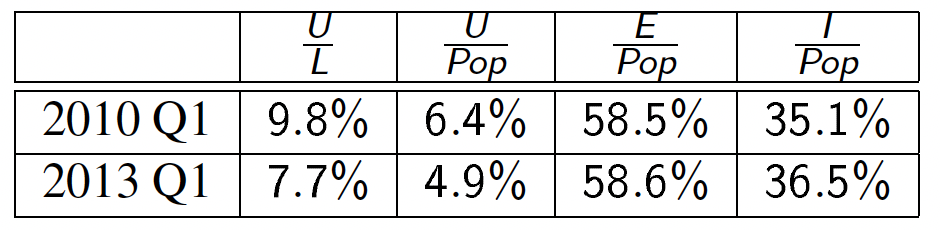
\includegraphics[width=7cm]{photos/2013 employment stats.png} }}%
    \qquad
    \subfloat[\centering 2010 Stats]{{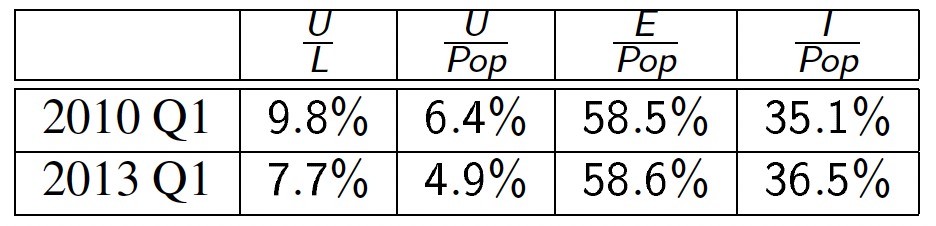
\includegraphics[width=7cm]{photos/2010 employment stats.png} }}%
    \caption{2010-2013: Unemployment and Employment stats}%
    \label{fig:2010-2013 employment stats}%
\end{figure}

\begin{figure}[h]
    \centering
    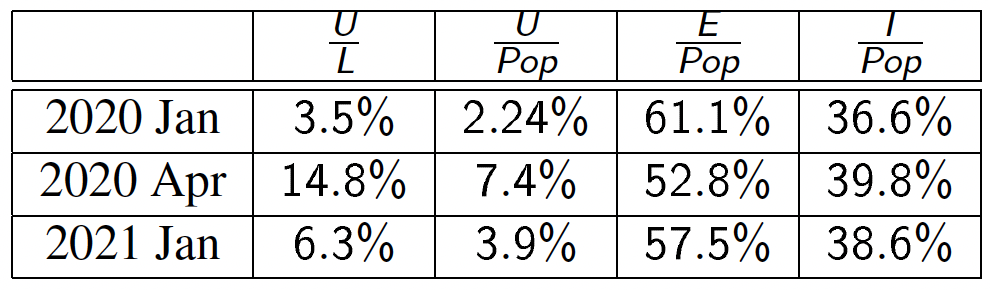
\includegraphics[width=7cm]{photos/2020 employmwnt stats.png}
    \caption{2020: Unemployment and Employment Throughout the Recession}
    \label{fig:2020 employment stats}
\end{figure}

\subsection{Theories of Unemployment}

Our neoclassical model explains \textit{why workers may decide to work more/fewer hours} $h$, \textit{how many weeks per year a worker chooses to work.} It does not explain \textbf{why someone who wants to work cannot find a job}. We must include friction in the model to break market clearing.

\subsubsection{Price Rigidity}

The simplest theory of unemployment comes from Keynesian price rigidities. Rigid wages cause labour markets not to clear.

\begin{figure}[h]
    \centering
    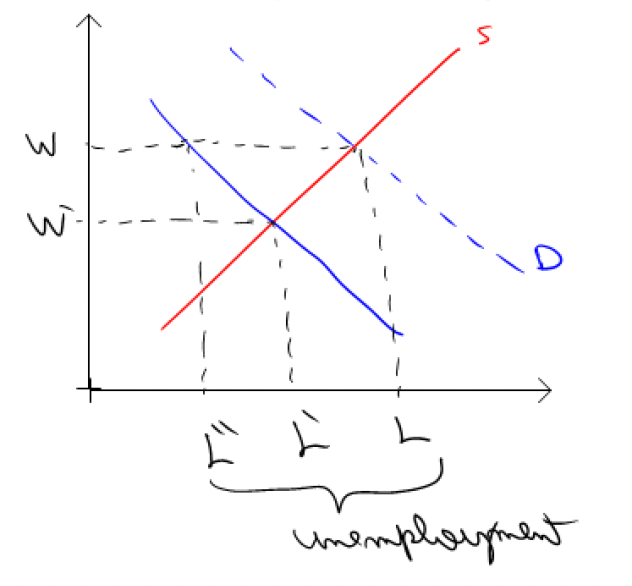
\includegraphics[width=10cm]{photos/rigid wages.png}
    \caption{Rigid Wages causing unemployment}
    \label{fig:rigid wages}
\end{figure}

At the macro level, it seems that average real wages fluctuate very little. But this may be clouded by \textbf{composition effects}.

\begin{intu}
        \textbf{Composition Effects}:

    Suppose there are two types of workers, high skill and low skill. Suppose that employment of low-skill workers is more volatile. In a recession, the share of low-skill workers will decrease. This would \hl{bias average wages upward}, even if the wages of high and low-skilled workers are going down individually.
\end{intu}

After controlling for this bias, wages are much more cyclical. Other authors have found different results.

This kind of theory is subject to the "Barro Critique":

\begin{definition}
    \textbf{Barro Critique:}

    Employers and unemployed workers would mutually benefit from agreeing to lower wages in this scenario. It makes it implausible that such wage rigidity would be sustained unless there were institutional constraints sustaining them (e.g. minimum wage).
\end{definition}

\subsubsection{Efficiency Wages}

This theory of unemployment comes from an informational hazard, \textbf{moral hazard}. When performing a task the workers choose the level of effort. But firms are not able to observe directly that level of effort. There is a probability the worker will get \textbf{caught shirking}.

\begin{shaded}
    \textbf{The model}:

    Take a 2-period version. Each period the worker's utility is given by
    \[u_t w_t - \epsilon_t\]
    where $w_t$ is the real wage, and $\epsilon_t$ is the level of effort. Workers have two options:

    \begin{enumerate}
        \item work $\epsilon>0$, implying $u = w - \epsilon$.

        \item Shirk: $\epsilon=0$, implying
        \begin{equation*}
            \left\{\begin{array}{cc}
            u = w & \text{if not caught} \\
            \text{ fired} & \text{if caught}
        \end{array} \right.
        \end{equation*}

        \begin{note}
            It is assumed that the firing happens in between periods.
        \end{note}
    \end{enumerate}
\end{shaded}

When will the worker exert effort? When the value of working $V$, is greater than the value of shirking $V^s$. So we must compute these values.

\begin{deriv}
    First, we calculate $V$, the value of working. We have:
    \begin{align*}
        V &= u_1 + \beta u_2 \\
        &= w - \epsilon + \beta\left[\delta V^U + (1-\delta)w\right]
    \end{align*}
    where $\beta$ controls for impatience. and $V^U$ is the value of unemployment

    Now, $V^s$. The shirker obtains $u_1 = w$ in the first period. However, if caught they lose their job in the second period. The shirker gets caught with probability $\theta$. Thus:

    \begin{align*}
        V^s &= u_1 + \beta u_2 \\
        &= w + \beta\left[(\delta+\theta)V^U + (1-\delta-\theta)w\right]
    \end{align*}
\end{deriv}
\begin{intu}
    Shirking gives you more value in period 1, but it increases the risk of losing your job in period 2.
\end{intu}

in this environment, firms want to pay the lowest wages that induce workers to put in effort.

\begin{figure}[h]
    \centering
    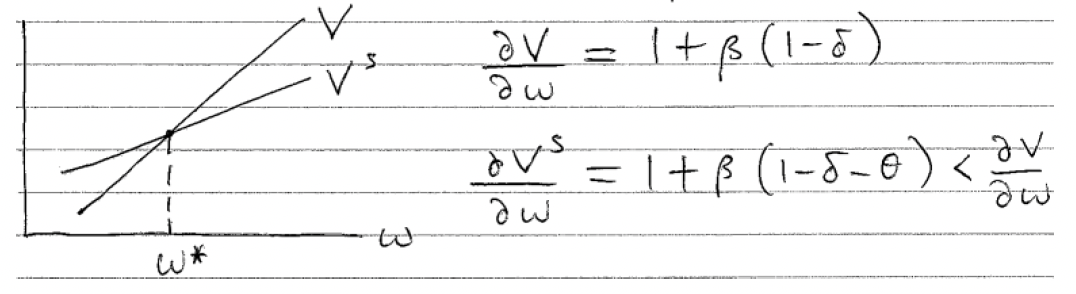
\includegraphics[width=10cm]{photos/v and v shirk.png}
    \caption{Finding the Efficient Wage where the Value of Working and Value of Shirking is Equal}
    \label{fig:efficient wage}
\end{figure}

We must find $w$ s.t $V=V^s$.

\begin{deriv}
We find $V=V^s$:
    \begin{equation}
    \label{derivation of efficient wage}
    \begin{aligned}
    w-\varepsilon+\beta\left[\delta V^U+(1-\delta) w\right]&=w+\beta\left[(\delta+\theta) V^U+(1-\delta-\theta) w\right] \\
    w+\beta(1-\delta) w-w-\beta(1-\delta-\theta) w&=\varepsilon-\beta \delta V^U+\beta(\delta+\theta) V^U \\
    \Rightarrow w &= V^U + \dfrac{\epsilon}{\beta\theta}.
\end{aligned}
\end{equation}
This is the so-called \hl{"no-shirking condition"} (NSC).
\end{deriv}

Now, we relate this to unemployment. We must compute $V^U$, the value of unemployment.
\begin{note}
    An unemployed worker finds a job with probability $f$.
\end{note}
Therefore, we have:
\[V^U = (1-f)b + fw\]
where $b$ reflects unemployment benefits, and the value of leisure.  If we combine this expression for $V^U$ and the NSC we get
\begin{mdframed}
    \begin{equation}
        \label{Aggregate NSC}
        \begin{aligned}
            w &= (1-f)b + fw + \dfrac{\epsilon}{\beta\theta} \\
            w &= b + \dfrac{1}{\beta(1-f)}\dfrac{\epsilon}{\theta}
        \end{aligned}
    \end{equation}

    This is the \textbf{aggregate NSC}.
\end{mdframed}

\begin{shaded}
    The model implies the following comparative statics:
    \begin{itemize}
        \item $b\uparrow \Rightarrow w\uparrow$ higher outside options require more pay to induce effort
        \item  $\epsilon\uparrow\Rightarrow w\uparrow$ The more costly effort is, the more pay is required.
        \item  $\theta\uparrow\Rightarrow w\downarrow$ The easier it is to monitor, the less pay is required
        \item $f\uparrow\Rightarrow w\uparrow$ If it is easier to find a job when unemployed, more rewards are needed.
        \item $\beta\uparrow\rightarrow w\downarrow$ The more patient people value the punishment more. This is because
    \end{itemize}
\end{shaded}

\subsubsection{Equilibrium Unemployment}

Let there be $L$ workers in the labour force. We can write changes in unemployment as:
\[\Delta U = \delta[L-U] - fU\]
\begin{note}
    In equilibrium, only exogenous job loss takes place.
\end{note}

In steady state, $\Delta U=0$, which implies
\[u = \dfrac{U}{L} = \dfrac{\delta}{\delta+f}\]

\begin{note}
    This can be rewritten as, $u\delta + uf = \delta$. Giving us:
    \[f(u) = \delta \dfrac{1-u}{u}\]
    where an increase in $u$ leads to a decrease in $f$. Higher rates of unemployment mean it is harder to find a job.
\end{note}

\begin{shaded}
    Final Efficiency Wages:

    Returning to NSC, we can write
    \[w = b \dfrac{1}{\beta[1-f(u)]}\dfrac{\epsilon}{\theta}\]

    Therefore, as $u\uparrow, f\downarrow, w^{NSC}\downarrow$. That is, as the rate of unemployment increases, it gets harder to find a job, and therefore our efficiency wage (NSC wage) decreases.
\end{shaded}

    \begin{figure}[h]
        \centering
        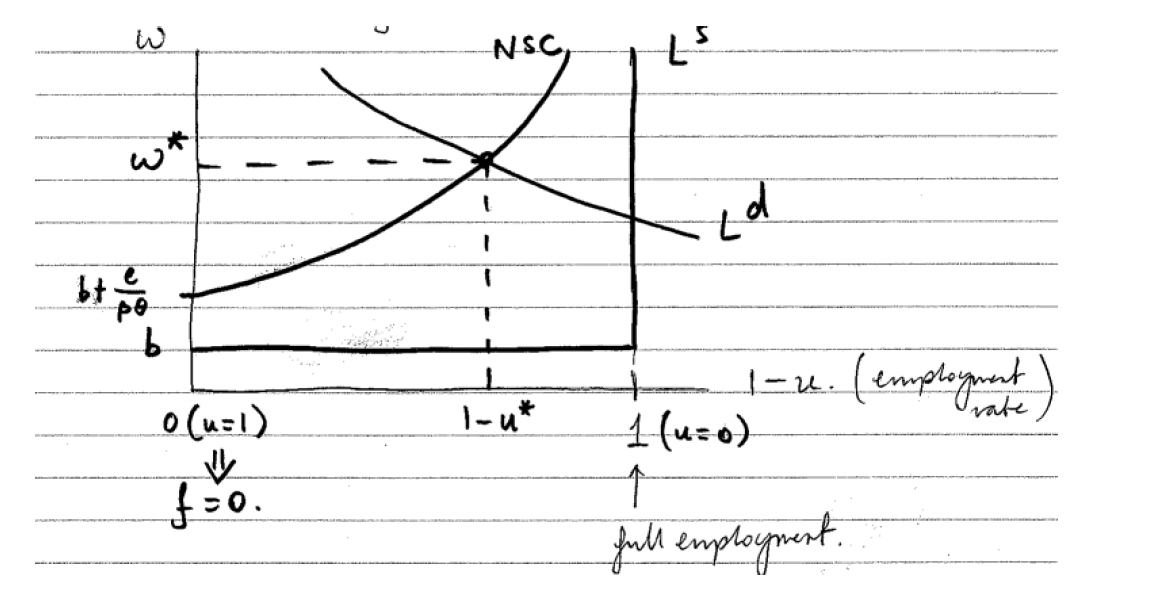
\includegraphics[width=10cm]{photos/NSC diagram.png}
        \caption{$L=N$ in this economy so employment rate equals $e = \frac{E}{N} = \frac{E}{L} = 1-u$}
        \label{fig:my_label}
    \end{figure}

    \begin{intu}
        The Shirking problem drives a wedge between labour demand and labour supply. This is driven by friction called moral hazard on behalf of the workers.
    \end{intu}

    \begin{shaded}
        Assessing the Shirking model:

        Pros:
        \begin{itemize}
            \item Can generate unemployment as an equilibrium phenomenon
        \end{itemize}
        Cons:
        \begin{itemize}
            \item The monitoring technology, $\theta$, it is hard to think that changes in this parameter help understand $\Delta u$.
            \item \textbf{Bonding Critique}: there are alternative payment arrangements involving bonds that would eliminate involuntary unemployment.
        \end{itemize}
    \end{shaded}

\section{Trade Union Model}

In this model, \textbf{workers} want higher wages via collective bargaining. Suppose the workers get together as a group to form a union and have a collective preference of the union $V^W$ given by
\[V^W = N^\gamma (w-V^U)\]
where $N$ is the number of workers, $w$ is the real wage, and $V^U$ is the value of unemployment. We can think of $w-V^U$ as the union premium, the additional utility you receive by being in the union.

The parameter $\gamma$ shapes the relative preference of the union between employment and higher wages. If $\gamma=0$ the union only cares about raising wages no matter what happens to employment.

\subsection{Right-to-manage}

\begin{shaded}
    In the right-to-manage framework, the union and the employer bargain over wages (Nash bargaining solution to determine wages). The employer sets employment unilaterally.

    The labour demand curve $N = N^D(w)$.
\end{shaded}

$w$ is the outcome of the following maximisation:
\begin{equation}
\begin{array}{r}
{\left[N^\gamma\left(w-V^U\right)\right]^\lambda \Pi(w)^{(1-\lambda)}} \\
\text { s.t. } N=N^d(w)
\end{array}
\end{equation}

where $\lambda$ is the bargaining power of the union, 0 implies no power, and $\Pi(.)$ is the profit function of the firm.

\begin{deriv}
    To solve for our Nash Product maximisation, we substitute the constraint in to the first equation.
    \begin{equation}
\max _w \lambda\left[\gamma \log \left(N^d(w)\right)+\log (\right.  \left.\left.w-V^U\right)\right] +(1-\lambda) \log (\Pi(w))
\end{equation}

We then find the FOC:
\begin{equation}
\lambda \gamma \frac{1}{N^d(w)} \frac{d N^d(w)}{d w}+\lambda \frac{1}{w-V^U}+(1-\lambda) \frac{1}{\Pi(w)} \frac{d \Pi(w)}{d w}=0
\end{equation}

multiplying by $w$ we have

\begin{equation}
\lambda \gamma \frac{w}{N^d(w)} \frac{d N^d(w)}{d w}+\lambda \frac{w}{w-V^U}+(1-\lambda) \frac{w}{\Pi(w)} \frac{d \Pi(w)}{d w}=0
\end{equation}

\begin{note}
    We must note the elasticities:

    The elasticity of employment w.r.t wage:
    \begin{equation}
        \label{elasticity of employment wrt wage}
        -\epsilon_N = \frac{w}{N^d(w)} \frac{d N^d(w)}{d w}
    \end{equation}

    The elasticity of profit w.r.t wage:
    \begin{equation}
        \label{elasticity of profit wrt wage}
        -\epsilon_\Pi = \frac{w}{\Pi(w)} \frac{d \Pi(w)}{d w}
    \end{equation}
\end{note}

Re-writing in terms of the elasticities:
\begin{equation}
    -\lambda\gamma\epsilon_N + \lambda \dfrac{w}{w-V^U}-(1-\lambda)\epsilon_\Pi = 0
\end{equation}
Then we solve for wage, $w$:
\begin{equation}
\begin{aligned}
\lambda w & =\left(w-V^U\right)\left[(1-\lambda) \varepsilon_{\Pi}+\lambda \gamma \varepsilon_N\right] \\
& \Longleftrightarrow \\
\lambda w-w\left[(1-\lambda) \varepsilon_{\Pi}+\lambda \gamma \varepsilon_N\right] & =-V^U\left[(1-\lambda) \varepsilon_{\Pi}+\lambda \gamma \varepsilon_N\right] \\
& \Longleftrightarrow \\
w & =\left[\frac{\lambda \gamma \varepsilon_N+(1-\lambda) \varepsilon_{\Pi}}{\lambda \gamma \varepsilon_N+(1-\lambda) \varepsilon_{\Pi}-\lambda}\right] V^u
\end{aligned}
\end{equation}

\begin{note}
    The bracketed term is greater than 1. Therefore we can re-write our equation simply as
    \begin{equation}
\begin{aligned}
w & =\left[\frac{\lambda \gamma \varepsilon_N+(1-\lambda) \varepsilon_{\Pi}}{\lambda \gamma \varepsilon_N+(1-\lambda) \varepsilon_{\Pi}-\lambda}\right] V^u \\
& =(1+\mu) V^u
\end{aligned}
\end{equation}
\end{note}

where $\mu>0$ is known as the \textbf{union mark-up}.
\end{deriv}

This means that workers are strictly better off than the unemployed, therefore for there to be unemployment it must be involuntary.

\subsubsection{Comparative Statics}

If we re-express our equation in terms of the markup, $\mu$.

\begin{equation}
\begin{aligned}
\mu & =\frac{\lambda \gamma \varepsilon_N+(1-\lambda) \varepsilon_{\Pi}}{\lambda \gamma \varepsilon_N+(1-\lambda) \varepsilon_{\Pi}-\lambda}-1 \\
& =\frac{\lambda \gamma \varepsilon_N+(1-\lambda) \varepsilon_{\Pi}-\lambda \gamma \varepsilon_N-(1-\lambda) \varepsilon_{\Pi}+\lambda}{\lambda \gamma \varepsilon_N+(1-\lambda) \varepsilon_{\Pi}-\lambda} \\
& =\frac{\lambda}{\lambda \gamma \varepsilon_N+(1-\lambda) \varepsilon_{\Pi}-\lambda} \\
& =\frac{1}{\gamma \varepsilon_N+\left(\frac{1-\lambda}{\lambda}\right) \varepsilon_{\Pi}-1}
\end{aligned}
\end{equation}

This gives us:
\begin{itemize}
    \item $\uparrow\lambda\Rightarrow\mu\uparrow$ If the union's bargaining power increases, the markup increases.
    \item  $\uparrow\gamma\Rightarrow\mu\downarrow$ If the union cares more about maintaining the employment of the workers, the markup will decrease.
    \item $\uparrow\epsilon_N \Rightarrow\mu\downarrow$, if the elasticity of employment wrt wages increases, the markup will decrease. 
    \item $\uparrow\epsilon_\Pi\Rightarrow\mu\downarrow$ If the elasticity of profits wrt wages increases, firms will be less willing to employ and therefore the markup will decrease.
\end{itemize}

Now we connect this to aggregate unemployment. We have considered the problem of a single firm/union. Now we create an economy that consists of many firms/unions. We still have the same value of unemployment
\[V^u = (1-f)b +fw\]

where $f$ is the probability of individuals finding a job, and $b$ is the payoff from unemployment. We combine this with the wage equation:

\[w = (1+\mu)[(1-f)b + fw]\]
solving for $w$

\begin{equation}
\begin{aligned}
w-(1+\mu) f w= & (1+\mu)(1-f) b \\
& \Longleftrightarrow \\
w & =\frac{(1+\mu)(1-f) b}{1-(1+\mu) f} \\
& =\frac{(1+\mu)(1-f) b}{1+\mu-(1+\mu) f-\mu} \\
& =\frac{(1+\mu)(1-f)}{(1+\mu)(1-f)-\mu} b
\end{aligned}
\end{equation}

where $f(u)=\delta\dfrac{1-u}{u}$, which implies an increase in unemployment leads to a decrease in the probability for unemployed workers to find a job, which decreases the wage.

The opposite of this gives us the union bargaining curve. That is, as unemployment decreases the job-finding rate increases, and wages increase.

\begin{figure}[h]
    \centering
    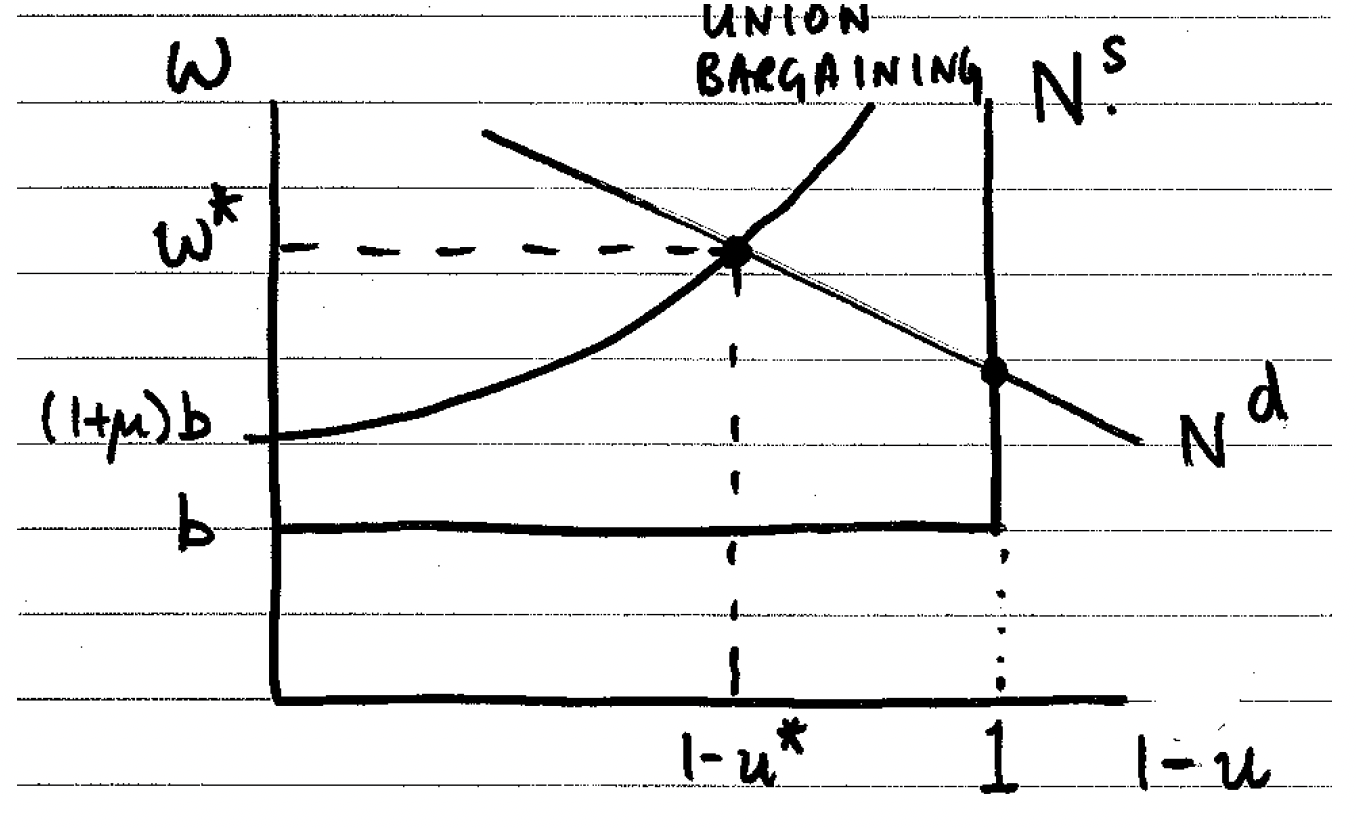
\includegraphics[width=12cm]{photos/union bargaining curve.png}
    \caption{Union Bargaining Curve}
    \label{fig:union bargaining curve}
\end{figure}

\begin{shaded}
    Assessing the Union Bargaining Model

    Pros: we have a coherent explanation of
    \begin{itemize}
        \item Why the equilibrium wage is greater than the market clearing wage
        \item Why the unemployed would like those jobs
        \item The existence of involuntary unemployment
    \end{itemize}
    Cons: the model seems inconsistent with the empirical evidence on Unions in Britain
    \begin{itemize}
        \item Unions were stronger in the 70s but lost power in the 80s and 90s. 
        \item Simultaneously, in the 80s unemployment increased.
    \end{itemize}
\end{shaded}


\section{Search Theory}

This model builds on the Diamond/Mortensen/Pissarides (DMP) model. This model is directly associated with the \textbf{flows approach} to labour markets, where we study the inflows and outflows of (un)employment.

We are explicitly taking into account the fact that the process of finding a job is \textbf{time-consuming} and a two-sided matching problem.

\begin{note}
    Unemployment naturally arises as the "normal" time for workers to find a suitable job.
\end{note}

In this theory, we focus on two employment states, unemployed (U), and employed (E). We neglect Inactive (I) because the changes to participation are quantitatively less important to explain fluctuations in THP at business cycle frequency.

\begin{shaded}
    There are two flows that are important

    $f$: the rate at which unemployed workers find jobs (outflow from unemployment)

    $s$: the rate at which employed workers lose their jobs (inflow to unemployment)

    This gives us
    \begin{align*}
      \Delta U &= sE - fU  \\
      &\Leftrightarrow \\
      \Delta u &= s(1-u) - fu
    \end{align*}
    \[\]
\end{shaded}

\subsection{Summary of Facts}

\begin{itemize}
    \item Both inflow and outflow rates are lower in Europe than in the US
    \item  This means that the US labour market is more "liquid"
    \item  Cyclical Variation: separations rise, and job finding reduces in recessions
    \item  Secular Variation: Large secular falls in $f$ in Europe in the 80s.
\end{itemize}

We want to build a model designed to explain the behaviour in $f$. In the US $f$ is quantitatively more important to explain $u$ over the business cycle.

\subsection{Properties of the Matching Function}

Job finding is the outcome of a \textbf{bilateral matching process between unemployed workers (U), and firm's vacancies (V)}. Several frictions make this process complicated. DMP summarise these complications into an aggregate matching function. Each period, $M(U,V)$ successful matches will take place.


\begin{itemize}
    \item $\dfrac{dM}{dU}>0, \dfrac{dM}{dV}>0$, and M is concave in each argument.
    \item M has constant returns to scale: $M(\alpha U, \alpha v) = \alpha M(U,V)$.
    \item This final assumption seems to hold in empirical tests.
\end{itemize}

\subsection{The model}

Given these assumptions, we can infer the matching rats:
\begin{itemize}
    \item Job-\textbf{Finding} rate, $f = \dfrac{M(U,V)}{U} = M(1,\frac{V}{U}) = f(\theta)$
    \item Job-\textbf{Filling} rate, $q = \dfrac{M(U,V)}{V} = M(\frac{U}{V},1) = q(\theta)$
\end{itemize}

where $\theta=\frac{V}{U}$ is the \textbf{labour market tightness}. When $\theta\uparrow$, there are more vacancies chasing fewer unemployed workers. This means that $f(]the
)\uparrow$ and $q(\theta)\downarrow$. It is harder for the firm to fill its vacancies. Higher market tightness is good for the worker.

We also introduce \textbf{Vacancy Costs}. To open a vacancy, firms must pay a cost of $c$. 

\begin{note}
    If there was free entry into vacancies, firms can open as many vacancies as they desire. As long as vacancies are profitable, firms would open infinite vacancies which would lead to \textit{zero unemployment}.
\end{note}

\paragraph{Additional Assumptions} \mbox{}

\begin{itemize}
    \item Firms hire workers through vacancies, each of which can hire one worker
    \item  When employed, a pair jointly produces \textbf{marginal product} $p$.
    \item  The unemployed receive \textbf{unemployment benefits}, $b$.
    \item We will look at a 1-period model.
\end{itemize}

To solve the model we need to determine the payoffs to workers and firms.

\begin{enumerate}
    \item Employed worker payoff:
    \[W_E = w\]

    \item  Unemployed worker payoff:
    \[W_u = (1-f(\theta)b + f(\theta)w\]

    \item productive firm payoff:
    \[\Pi_F = p-w\]

    \item  Vacancy payoff:
    \[\Pi_V = -c + q(\theta)(p-w) + \underset{=0}{\underbrace{(1-q(\theta))0}}\]
\end{enumerate}

\paragraph{Job Creation Condition}\mbox{}

Because we assume free entry, the value of a vacancy $\Pi_V$ is driven to 0. This implies 
\begin{gather*}
    -c + q(\theta)(p-w) = 0 \\
    \Leftrightarrow \\
    \Pi_F = p-w=\dfrac{c}{q(\theta)} \\
    \Leftrightarrow \\
    w-p = -\dfrac{c}{q(\theta)}
\end{gather*}

Therefore, an increase in market tightness, $\uparrow\theta$, leads to a decrease in the job-filling rate, $q(\theta)\downarrow$, which leads to a decrease in wage $w \downarrow$.

This is called the \textbf{Job Creation Condition} (JC). It is analogous to the labour demand curve in the neoclassical model.


\paragraph{Wage-Bargaining Condition}

We must close the model, so we find a wage-setting mechanism that relates $w$ to $\theta$.

\begin{note}
    A search problem entails \textbf{ex-post rents} to employed workers and firms, i.e. it is costly for a firm to find an alternative worker: $-c<p-w$, and $q(\theta)<1$. Also, it is costly for the workers to find an alternative firm: $b<w$, and $f(\theta)<1$.
\end{note}

Wages determine the split of rents (the surplus) between workers and firms. In the DMP we assume the rents are split via Nash Bargaining. Additionally, we will assume that the firm and workers have equal bargaining power, and thus the rents are split equally.

\[\Pi_F - \Pi_V = W_E - W_U\]
Because in equilibrium the value of vacancies is driven to 0, this is simply
\[W_E - \Pi_F = W_U\].

\begin{deriv}
    On the LHS we have:
   \begin{equation}
W_E-\Pi_F=w-(p-w)=2 w-p
\end{equation}

RHS:
\begin{equation}
\begin{aligned}
W_U & =(1-f) b+f W_E \\
& =(1-f) b+f\left(W_E-W_U\right)+f W_U \\
& =(1-f) b+f \frac{c}{q}+f W_U \\
\text{we are using the fact that: } &W_E - W_U = \Pi_F = \frac{c}{q} \\
W_U - fW_U &= (1-f)b + f\frac{c}{q} \\
W(1-f) &= (1-f)b + f\frac{c}{q} \\
W_U &= b + \dfrac{f(\theta)}{1-f(\theta)}\dfrac{c}{q(\theta)}
\end{aligned}
\end{equation}

Equating the LHS and RHS, we have:
\begin{align*}
    2w-p &= b + \dfrac{f(\theta)}{1-f(\theta)}\dfrac{c}{q(\theta)} \\
    \Leftrightarrow& \\
    w&= \dfrac{1}{2}p + \dfrac{1}{2}b + \dfrac{1}{2}\dfrac{f(\theta)}{1-f(\theta)}\dfrac{c}{q(\theta)}
\end{align*}
This is the \textbf{Wage Bargaining Conditions}
.\begin{note}
    We have all halves here because the firm and workers have equal bargaining power.
\end{note}
\end{deriv}

\newpage
\begin{shaded}
    \paragraph{Comparative Statics} \mbox{}

    \begin{gather*}
        p\uparrow\Rightarrow w\uparrow \\
        b\uparrow \Rightarrow w\uparrow \\
        c\uparrow\Rightarrow w \uparrow \\
        \theta\uparrow \Rightarrow q(\theta)\downarrow, f(\theta)\uparrow \Rightarrow w\uparrow
    \end{gather*}

    An increase in market tightness makes it easier for workers to find jobs. Therefore, the outside option goes up in negotiation.
\end{shaded}

We have our model equilibrium:

\begin{figure}[h]
    \centering
    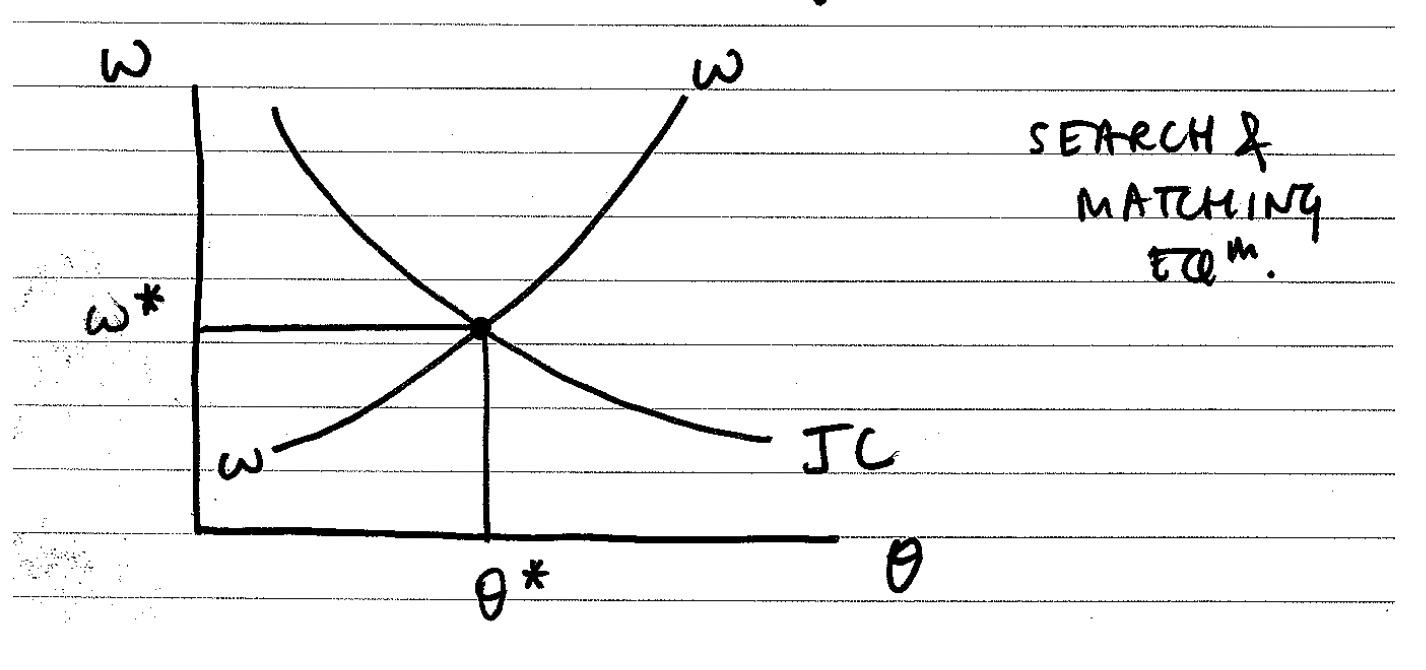
\includegraphics[width=12cm]{photos/search and matching equilibrium.png}
    \caption{Search and Matching Equilibrium. Our Wage Setting and Job Creation Conditions}
    \label{fig:search and matching equilibrium}
\end{figure}

\section{Analysis of the DMP model}

We determined equilibrium wages, $w^*$ and tightness, $\theta^*$. This gives us
\[f^* = f(\theta^*) = M(1,\theta^*), \quad q^* = q(\theta^*) = M(\frac{1}{\theta^*},1)\]

In steady state, $u^* = \dfrac{s}{s+f^*}$

\subsection{Application to the Business Cycle}

We will represent the real business cycles as shocks to real productivity, $p$, which drive the cycle.

Our Equilibrium Conditions were:

\begin{equation}
\begin{aligned}
\mathrm{JC} w & =p-\frac{c}{q(\theta)} \\
\mathrm{WB} w & =\frac{1}{2} p+\frac{1}{2} b+\frac{1}{2} \frac{f(\theta)}{1-f(\theta)} \frac{c}{q(\theta)}
\end{aligned}
\end{equation}

By equating the two we find $\theta^*$. We can see that shocks to $p$ have differing effects on each of the curves, due to the coefficient.

\begin{figure}[h]
    \centering
    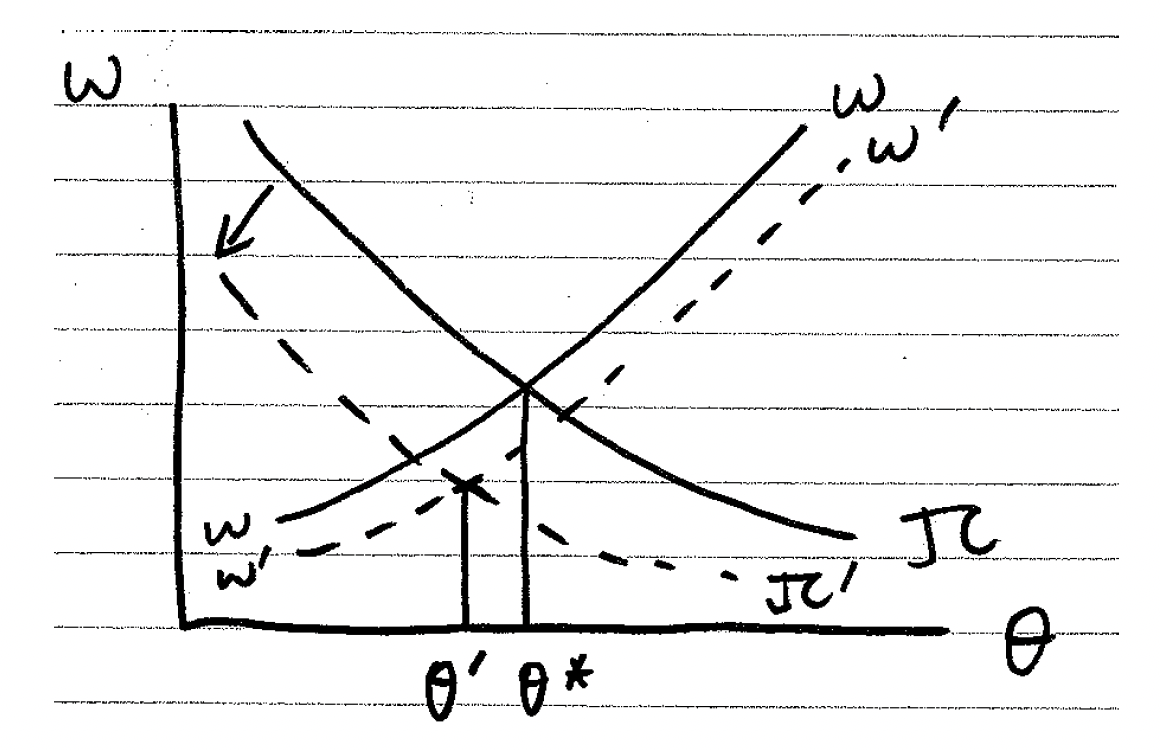
\includegraphics[width=12cm]{photos/shock to p DMP.png}
    \caption{Result of a shock to real Productivity}
    \label{fig:DMP shock p}
\end{figure}

$p \downarrow \Longrightarrow \theta^* \downarrow \Longrightarrow f\left(\theta^*\right) \downarrow \Longrightarrow u^*=\frac{s}{s+f^*} \uparrow$. This result is not ambiguous.

\begin{equation}
\begin{gathered}
\frac{1}{2} p+\frac{1}{2} b+\frac{1}{2} \frac{f(\theta)}{1-f(\theta)} \frac{c}{q(\theta)}=p-\frac{c}{q(\theta)} \\
\frac{1}{2} b+\frac{1}{2} \frac{f(\theta)}{1-f(\theta)} \frac{c}{q(\theta)}+\frac{c}{q(\theta)}=\frac{1}{2} p
\end{gathered}
\end{equation}
LHS is increasing in $\theta$. Thus, this equation implies that increases in $p$ lead to increases in $\theta$.

\subsection{DMP Implications on Vacancies}

In the steady state, matches destroyed (jobs lost) must be equal to the number of new matches
\[s(1-u) = M(u,v)\]

Thus, if $u\downarrow \Rightarrow LHS\uparrow$ 
 and $RHS\downarrow$, therefore, $v$ must increase to keep equality. Therefore, as the unemployment rate decreases, vacancies increase, meaning that vacancies are \textbf{pro-cyclical}. This equation defines the \textbf{Beveridge Curve}.

 \begin{figure}[h]
     \centering
     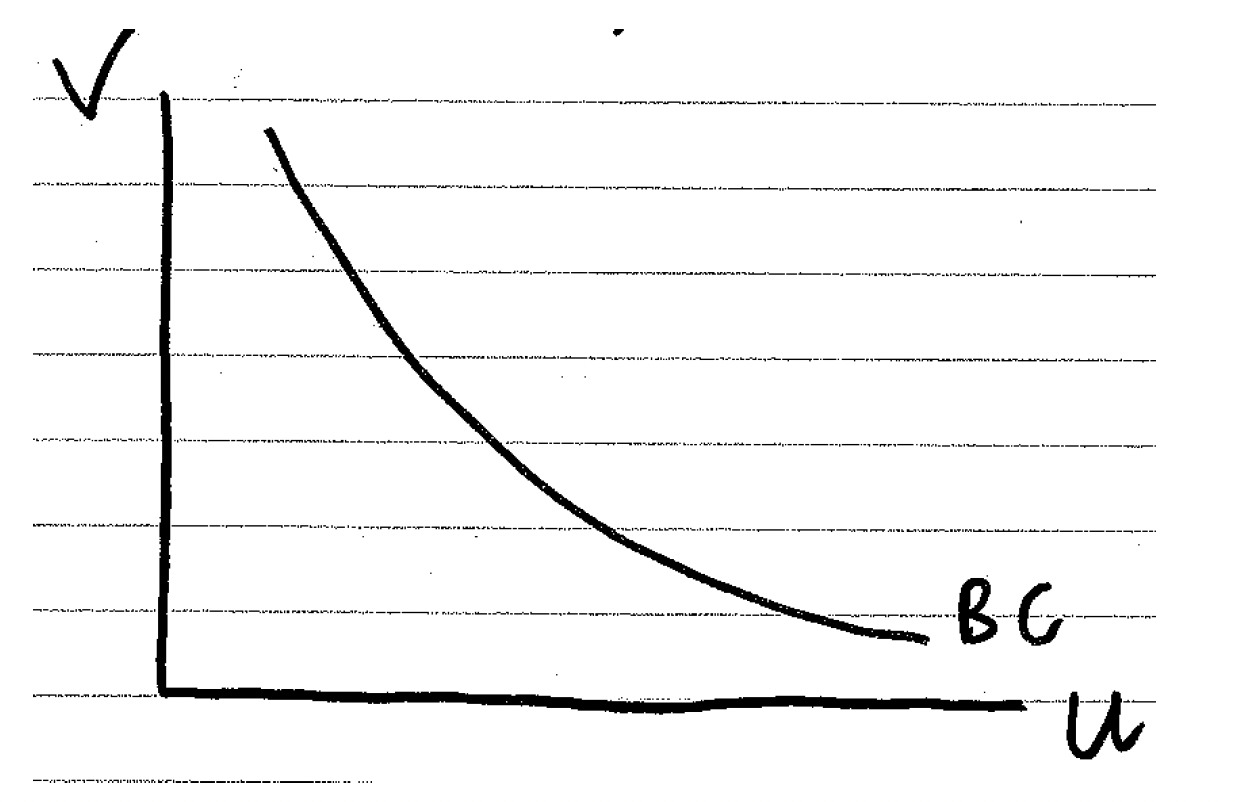
\includegraphics[width=12cm]{photos/bc curve.png}
     \caption{Beveridge Curve}
     \label{fig:BC curve}
 \end{figure}
Using the $\theta^*$ from our Job Creation and Wage setting conditions, we can draw a line with \textbf{angle} $\theta$. Where this line intersects the BC, will be the equilibrium vacancy and unemployment rates.

 This curve came from real-life data. So, we have seen that the model can \textbf{qualitatively} explain unemployment over the business cycle, but what about quantitatively?

 \subsection{Model for cyclical nature of Job finding Rate}


$f$ is a very pro=cyclical variable. 1\% increase in productivity leads to a 5\% increase in $f$.

Our solution for $\theta$ is
\begin{equation}
\frac{1}{2} b+\frac{1}{2} \frac{f(\theta)}{1-f(\theta)} \frac{c}{q(\theta)}+\frac{c}{q(\theta)}=\frac{1}{2} p
\end{equation}
and therefore:
\begin{equation}
\frac{d f}{d p} \frac{p}{f}=\frac{f^{\prime}(\theta) \theta}{f} \frac{d \theta}{d p} \frac{p}{\theta}
\end{equation}

Now, in order to compute elasticities, we must make a functional form assumption about $M(U,V) = \frac{UV}{U+V}$.
\begin{note}
    We have CRS in the matching function.
\end{note}

We have most of the elements in Equation (75):

\begin{gather}
    f(\theta) = M(1,\theta) = \dfrac{\theta}{1+\theta} \\
    q(\theta) = M(\frac{1}{\theta},1) = \dfrac{\frac{1}{\theta}}{\frac{1}{\theta}+1} = \dfrac{1}{1+\theta} \\
    f^\prime(\theta) = \dfrac{1}{1+\theta}-\dfrac{\theta}{(1+\theta)^2}=\dfrac{1}{(1+\theta)^2}\\
    \dfrac{f^\prime(\theta)\theta}{f}= \dfrac{\theta}{(1+\theta)^2}\dfrac{1+\theta}{\theta} = \dfrac{1}{1+\theta}
\end{gather}

thus, we only need to compute $\dfrac{d\theta}{dp}\dfrac{p}{\theta}$. Substituting in $f(\theta)$ and $q(\theta)$:

\begin{equation}
\begin{gathered}
 \frac{1}{2} b+\frac{1}{2} \dfrac{\frac{\theta}{1+\theta}}{1-\frac{\theta}{1+\theta}} c(1+\theta)+c(1+\theta)=\frac{1}{2} p \\
 \dfrac{\frac{\theta}{1+\theta}}{\frac{1+\theta-\theta}{1+\theta}} c(1+\theta)+2 c(1+\theta)=p-b \\
  \Longleftrightarrow \\
 c(1+\theta)(2+\theta)=p-b \\
\end{gathered}
\end{equation} 

Differentiating both sides wrt $p$ we have:
\[c(2+\theta) \dfrac{d\theta}{dp} + c(1+\theta)\dfrac{d\theta}{dp} = 1\]

which gives:
\[\dfrac{d\theta}{dp}=\dfrac{1}{c(3+2\theta)}\]


\begin{note}
It is difficult to obtain estimates of $c$, so we will continue.
\end{note}


\begin{equation}
\begin{aligned}
\frac{d \theta}{d p} \frac{p}{\theta} & =\frac{1}{c(3+2 \theta)} \frac{p}{\theta} \\
& =\frac{p}{c \theta(3+2 \theta)} \frac{p-b}{p-b} \\
& =\frac{c(1+\theta)(2+\theta)}{c \theta(3+2 \theta)} \frac{p}{p-b} \\
& =\frac{(1+\theta)(2+\theta)}{\theta(3+2 \theta)} \frac{1}{1-\frac{b}{p}}
\end{aligned}
\end{equation}

where we have used Equation (80) ($p-b = c(1+\theta)(2+\theta)$.

it is possible to provide reasonable numbers for $\theta=1$ and $\frac{b}{p}=0.4$. This implies
\begin{itemize}
    \item $\dfrac{d\theta}{dp}\dfrac{p}{\theta}\approx 2$
    \item $\frac{d f}{d p} \frac{p}{f}=\frac{f^{\prime}(\theta) \theta}{f} \frac{d \theta}{d p} \frac{p}{\theta}=\frac{1}{1+\theta} \frac{d \theta}{d p} \frac{p}{\theta} \approx 1$
\end{itemize}

\begin{note}
    Our elasticity is much less than the empirical findings of 5. this model severely underestimates fluctuations in $f$.
\end{note}


\subsection{Hall (2005) Model}

Hall proposes wage rigidity. We had been assuming that wages are set through Nash Bargaining, but now we are not. What are the bounds for the possible \textbf{acceptable} wages?

\begin{enumerate}
    \item Lowest Acceptable Wage: Worker is indifferent between working or not
    \[W_E = \underline{w} = (1-f(\theta)\]
\end{enumerate}

\begin{enumerate}
    \item Lowest Acceptable Wage: Worker is indifferent between working or not
    \[W_E = \underline{w} = (1-f(\theta)\underline(w) = W_U\]
therefore, $\underline{w} = b$


    \item  Maximum acceptable wage: Firms earn zero profit
\[\Pi_F = p - w = 0 = \Pi_V \]
Therefore, $w = p$
\end{enumerate}

We know that any $w \in [b,p]$ is a possible outcome

\paragraph{Hall's Solution}\mbox{}

Wages follow a "norm" and remain unchanged over time. \hl{The Barro critique does not apply here since it is a feasible outcome from bargaining}.

\begin{figure}[h]
\centering
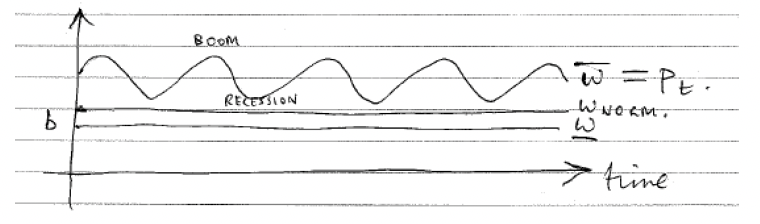
\includegraphics[width=10cm]{photos/halls solution.png}
\caption{Hall's Solution where wages follow a "norm".}
\label{fig: Halls solution}
\end{figure}


\subsubsection{Applying Wage Norms to DMP}

\begin{figure}[h]
    \centering
    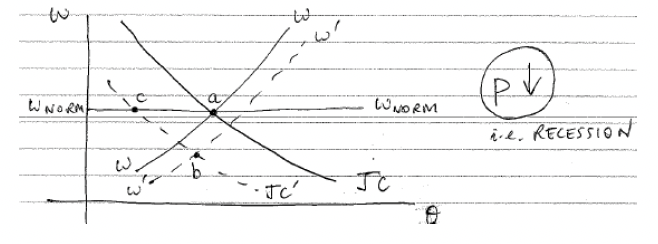
\includegraphics[width=10cm]{photos/applying rigid wage.png}
    \caption{The effect of a recession when there are wage "norms"}
    \label{fig: applied wage norms}
\end{figure}

In our normal case where wages are set through Nash Bargaining, we would move from point a to b. in the case where we have a wage norm, we move from a to c. 


\paragraph{Quantitatively} \mbox{}

\begin{deriv}
JC equals $w_{norm}$:
\[p - \dfrac{c}{q(\theta)} = w_{norm} \]

Differentiating wrt $p$:
\begin{equation}
\begin{aligned}
\dfrac{d\theta}{sp}\dfrac{p}{\theta}& = \dfrac{1}{c}\dfrac{p}{\theta} =  \dfrac{1}{c}\dfrac{p}{\theta}\dfrac{p-w_{norm}}{p-w_{norm}} \\
&= \dfrac{1+\theta}{\theta}\dfrac{P}{p-w_{norm}}
\end{aligned}
\end{equation}

where we used the fact that $p-w_{norm}=\frac{c}{q(\theta)}=c(1+\theta)$.

\end{deriv}
 This gives us

\[\dfrac{df}{sp}\dfrac{p}{f} = \dfrac{1}{\theta}\dfrac{1}{1-\frac{w_{norm}}{P}}\]

If $\theta=1$ and $\frac{w_{norm}}{P}=0.8$, then our elasticity $\frac{df}{dp}\approx 5$ like the data.


\begin{shaded}
\paragraph{Evaluating the Hall model} \mbox{}

Pros:
\begin{itemize}
\item Provides theory that explains variations in unemployment over the business cycle
\item The element of wage rigidity is not subject to Barro's critique.
\end{itemize}

Cons:
\begin{itemize}
\item Wages of \textbf{new hires} have to be rigid for a firm.
\item There is mixed evidence of wage rigidity in the data. Both for new hires and outgoing matches.
\end{itemize}

\end{shaded}









\end{document}
